\setcounter{section}{0}% Set chapter counter
%\numberwithin{equation}{chapter}% Equation counter follows chapter
\numberwithin{equation}{section}% Equation counter follows section

\setcounter{chapter}{0}

\chapter{\texorpdfstring{A first look at strings}{1 A first look at strings}} \label{cha:1} 

\section{\texorpdfstring{Why strings?}{Why strings?}}
String theory is an ambitious attempt to provide a unified "Theory of Everything," incorporating all fundamental forces of nature—gravity, electromagnetism, and the nuclear forces—into a single quantum mechanical framework. The primary motivation for this shift from standard physics lies in the inherent limitations of Quantum Field Theory (QFT) when applied to gravity.

In QFT, elementary particles are treated as zero-dimensional points. This assumption leads to severe ultraviolet (UV) divergences because interactions occur at a single point in spacetime, resulting in mathematical singularities. While theories like the Standard Model can be "renormalized" to manage these infinities, point-particle gravity is famously non-renormalizable. At the Planck scale ($10^{-33}$ cm), the point-particle description of gravitational interactions simply breaks down.


String theory solves this problem by replacing point-like particles with one-dimensional loops and strands of string. This extension "smears out" interactions in spacetime. From a worldsheet perspective, what appears as a sharp, singular vertex in point-particle diagrams becomes a smooth, continuous topology in string theory. This smoothing effectively removes the UV divergences that plague point-particle gravity.

Furthermore, string theory is a uniquely constrained theory. It does not just allow for gravity; it necessitates it. The spectrum of string excitations naturally includes a massless spin-2 particle, which is identified as the graviton. Thus, general relativity emerges as a necessary low-energy consequence of the theory rather than an added assumption. 

While the theory requires higher dimensions (e.g., $D=26$ for the bosonic string) to maintain Lorentz invariance, it remains our most promising route toward a complete and consistent unification of the physical laws.

\section{\texorpdfstring{Action principles}{Action principles}} \label{sec:1.2}
The string moves in $D$-dimensional flat spacetime with metric $\eta_{\mu\nu}=\operatorname{diag}(-,+,+,\cdots,+)$. 

First, let us review the classical mechanics of a zero-dimensional object. 
For a relativistic point particle, we can describe it using $D-1$ positions as functions of time $\textbf{X}(X^0)$. However, this hides the covariance of the theory. 
Therefore, it is better to introduce a parameter $\tau$ along the particle's worldline and describe the motion in spacetime with $D$ functions $X^\mu(\tau)$. The parameterization is arbitrary: different parameterizations of the same path are physically equivalent. That is, for any monotonic function $\tau^\prime(\tau)$, the two paths are identical: 
\begin{equation}
	X^{\prime\mu}(\tau^\prime(\tau))=X^\mu(\tau)
\end{equation}
The simplest Poincaré-invariant action (which does not depend on the parameterization) is proportional to the proper time along the worldline: 
\begin{equation}
	S_{\mathrm{pp}}=-m \int \dif\tau\:(-\dot{X}^\mu \dot{X}_\mu)^{1/2}
\end{equation}
where $\dot{X}^\mu=\frac{\partial X^\mu}{\partial \tau}$. 
The variation of the action (after integration by parts) is: 
\begin{equation}
	\delta S_{\mathrm{pp}}=+m \int \dif\tau\: \tfrac{1}{2}(-\dot{X}^\nu \dot{X}_\nu)^{-1/2}\, 2\dot{X}_\mu \delta\dot{X}^\mu=m \int \dif\tau\: u_\mu \delta \dot{X}^\mu \nonumber\:,
\end{equation}
so 
\begin{equation}
	\delta S_{\mathrm{pp}}=-m \int \dif\tau\: \dot{u}_\mu \delta X^\mu
\end{equation}
where 
\begin{equation}
	u^\mu=\dot{X}^\mu (-\dot{X}^\nu \dot{X}_\nu)^{-1/2}
\end{equation}
is the normalized $D$-velocity. 
Thus, the equation of motion $\dot{u}^\mu=0$ describes free motion. The normalization constant $m$ is the particle mass. 

By introducing an auxiliary field on the worldline, a worldline-independent metric $\gamma_{\tau\tau}(\tau)$, this action can be transformed into another form. It is convenient to use the einbein $\eta(\tau)=(-\gamma_{\tau\tau}(\tau))^{1/2}$. This is defined to be positive-definite. We use the General Relativity term "tetrad" in any dimension (even though its root means "4"). Then: 
\begin{equation}
	S^\prime _{\mathrm{pp}}=\frac{1}{2}\int \dif\tau\: \Bigl(\eta^{-1}\dot{X}^\mu \dot{X}_\mu-\eta m^2\Bigr) \label{action-reparameter}
\end{equation}
This action has the same symmetries as $S_{\mathrm{pp}}$, namely Poincaré invariance and reparameterization invariance. 
\begin{tcolorbox}[breakable]
	\begin{proof}
		The standard action for a free relativistic massive point particle is proportional to the invariant proper time along its worldline. The Lagrangian is given by:
		\begin{align*}
			L &= -m\sqrt{-\dot{x}^2} = -m\sqrt{-\dot{x}^\mu \dot{x}_\mu}
		\end{align*}
		where $\dot{x}^\mu = \frac{dx^\mu}{d\tau}$ is the four-velocity with respect to an arbitrary worldline parameter $\tau$, and we adopt the mostly-plus metric signature $(-, +, +, +)$.
		
		To transition to the Hamiltonian formalism, we must perform a Legendre transformation. We first compute the canonical momenta conjugate to the coordinates $x^\mu$:
		\begin{align*}
			p_\mu &= \frac{\partial L}{\partial \dot{x}^\mu} = \frac{m\dot{x}_\mu}{\sqrt{-\dot{x}^2}} \implies p^2 = p^\mu p_\mu = \frac{m^2 \dot{x}_\mu \dot{x}^\mu}{-\dot{x}^2} = -m^2
		\end{align*}
		
		In a standard, non-constrained system, the next step is to invert this relation to express the velocities $\dot{x}^\mu$ as functions of the coordinates and momenta. However, this Legendre transformation is \textbf{non-invertible}. Mathematically, this non-invertibility manifests because the Hessian matrix of the Lagrangian with respect to the velocities is singular:
		\begin{align*}
			\det \left( \frac{\partial^2 L}{\partial \dot{x}^\mu \partial \dot{x}^\nu} \right) &= 0
		\end{align*}
		
		Instead of an invertible relationship, squaring the canonical momentum yields an algebraic identity relating the momenta themselves, giving the momentum constraint $p^\mu p_\mu + m^2 = 0$. In Dirac's theory of constrained Hamiltonian systems, this is known as a \textbf{primary constraint}. 
		
		Next, we calculate the canonical Hamiltonian, $H_c$:
		\begin{align*}
			\dot{x}^\mu p_\mu &= \dot{x}^\mu \left( \frac{m\dot{x}_\mu}{\sqrt{-\dot{x}^2}} \right) = -m\sqrt{-\dot{x}^2} = L \implies H_c = 0
		\end{align*}
		The canonical Hamiltonian vanishes identically ($H_c = 0$), which is a universal feature of fully reparametrization-invariant theories. 
		
		Because the Legendre transformation is non-invertible and the canonical Hamiltonian vanishes, we must incorporate the primary constraint into our Lagrangian formalism via a Lagrange multiplier, $\eta$, to restore dynamics:
		\begin{align*}
			L &= \dot{x}^\mu p_\mu - \frac{\eta}{2}(p^2 + m^2) - H_c \quad (\text{where } H_c=0)
		\end{align*}
		
		From the equation of motion (EoM) for $p_\mu$:
		\begin{align*}
			\left( \frac{\partial L}{\partial p_\mu} \right) - \frac{d}{d\tau}\left( \frac{\partial L}{\partial \dot{p}_\mu} \right) = 0 &\implies \dot{x}^\mu - \eta p^\mu = 0 \\
			&\implies p^\mu = \frac{1}{\eta}\dot{x}^\mu
		\end{align*}
		
		We can now cleanly eliminate $p^\mu$ from the action to get the second-order form:
		\begin{align*}
			L &= \dot{x}^\mu\left(\frac{\dot{x}_\mu}{\eta}\right) - \frac{\eta}{2}\left( \left(\frac{\dot{x}}{\eta}\right)^2 + m^2 \right) \\
			&= \frac{\dot{x}^2}{\eta} - \frac{\dot{x}^2}{2\eta} - \frac{\eta}{2}m^2 \\
			&= \frac{1}{2}\left(\frac{\dot{x}^2}{\eta} - \eta m^2\right)
		\end{align*}
		This final expression is the Polyakov action (or einbein action) for the point particle. By introducing the Lagrange multiplier $\eta(\tau)$ to manage the non-invertible Legendre transformation, we have arrived at an equivalent formulation that avoids the troublesome square root and seamlessly accommodates massless particles $(m=0)$.
	\end{proof}
\end{tcolorbox}
For the latter, the transformation of $\eta(\tau)$ is: 
\begin{equation}
	\eta^\prime(\tau^\prime)\dif\tau^\prime=\eta(\tau)\dif\tau\:
\end{equation}
\begin{tcolorbox}[breakable]
	\begin{proof}
		\begin{align*}
			S^\prime _{\mathrm{pp}}&=\frac{1}{2}\int \dif\tau\: \Bigl(\eta^{-1}\dot{X}^\mu \dot{X}_\mu-\eta m^2\Bigr) \nonumber \\
			&=\frac{1}{2}\int \dif\tau^\prime \:\Bigl(\frac{\dif\tau}{\dif\tau^\prime} \eta^{-1}\frac{\partial X^\mu}{\partial \tau} \frac{\partial X_\mu}{\partial \tau}-\frac{\dif\tau}{\dif\tau^\prime} \eta m^2\Bigr) \nonumber \\
			&=\frac{1}{2}\int \dif\tau^\prime\: \biggl(\frac{\dif\tau}{\dif\tau^\prime} \eta^{-1}\Bigl(\frac{\dif\tau^\prime}{\dif\tau}\Bigr)^2\frac{\partial X^\mu}{\partial \tau^\prime} \frac{\partial X_\mu}{\partial \tau^\prime}- \eta^\prime m^2\biggr) \nonumber \\
			&=\frac{1}{2}\int \dif\tau^\prime\: \Bigl(\eta^{\prime -1}\frac{\partial X^\mu}{\partial \tau^\prime} \frac{\partial X_\mu}{\partial \tau^\prime}- \eta^\prime m^2\Bigr) \nonumber
		\end{align*}
	\end{proof}
\end{tcolorbox} 

Varying with respect to the einbein $\eta(\tau)$ yields the equation of motion: 
\begin{align}
	&\delta S_{\mathrm{pp}}^\prime =\frac{1}{2}\int \dif\tau\:\Bigl(-\frac{1}{\eta^{-2}}\dot{X}^\mu\dot{X}_\mu-m^2\Bigr)\delta\eta \nonumber \\
	&\Longrightarrow \eta^2=-\dot{X}^\mu\dot{X}_\mu/m^2 \label{1.2.7}
\end{align}
Using this to eliminate $\eta$ from (\ref{action-reparameter}), $S_{\mathrm{pp}}^\prime$ becomes $S_{\mathrm{pp}}$. 
$S_{\mathrm{pp}}^\prime$ can handle massless particles, whereas $S_{\mathrm{pp}}$ cannot. 
Although $S_{\mathrm{pp}}^\prime$ and $S_{\mathrm{pp}}$ are classically equivalent, $S_{\mathrm{pp}}$ is difficult to path-integrate due to its complicated form. Conversely, $S_{\mathrm{pp}}^\prime$ is a quadratic in derivatives, making the path integral quite easy to compute. One can infer that any attempt to define a quantum theory for $S_{\mathrm{pp}}$ will lead to results equivalent to the path integral of $S_{\mathrm{pp}}^\prime$. We take the latter as the starting point for the quantum theory. 

A one-dimensional object sweeps out a two-dimensional worldsheet, described by two parameters, denoted $X^\mu(\tau, \sigma)$. We still insist that the action depends only on the embedding in spacetime, not on the parameterization. The simplest action is the Nambu-Goto action, which is proportional to the area of the worldsheet. 
Introduce the induced metric $h_{ab}$, where $a,b$ range over $(\tau, \sigma)$: 
\begin{equation}
	h_{ab}\equiv\pdv{X^{\mu}}{x^a}\pdv{X^{\nu}}{x^b}\eta_{\mu\nu}=\partial_a X^\mu\partial_b X_\mu
\end{equation}
Then the Nambu-Goto action is: 
\begin{subequations} \label{1.2.9} % 
	\begin{align}
		S_{\mathrm{NG}}&=\int_M \dif\tau \dif\sigma\: \mathscr{L}_{NG} \\
		\mathscr{L}_{\mathrm{NG}}&=-\frac{1}{2\pi\alpha^\prime}(-\det h_{ab})^{1/2}
	\end{align} 
\end{subequations}
where $M$ represents the worldsheet, and $\alpha^\prime$ has dimensions of $L^2$, representing the Regge slope. The relationship between the string tension $T$ and the Regge slope is: 
\begin{equation}
	T=\frac{1}{2\pi\alpha^\prime}
\end{equation}
Now consider the symmetries of this action. 
Transformations of $X^\mu(\tau, \sigma)$ that satisfy $S_{\mathrm{NG}}(X^\prime)=S_{\mathrm{NG}}(X)$ include: 
\begin{enumerate}
	\item Isometry group of flat spacetime ($D$-dimensional Poincaré group): 
	\begin{equation}
		X^{\prime \mu}(\tau,\sigma)=\Lambda^{\mu}{}_{\nu} \,X^\nu(\tau,\sigma)+a^\mu.
	\end{equation} 
	\item Two-dimensional coordinate invariance (called diffeomorphism invariance, abbreviated as diff): 
	\begin{equation}
		X^{\prime \mu}(\tau^\prime,\sigma^\prime)=X^{\mu}(\tau,\sigma).
		\label{diffeomorphism}
	\end{equation} 
\end{enumerate}
\begin{tcolorbox}[breakable]
	\begin{remark}
		The worldsheet coordinates do not have any inherent physical meaning, just like the worldline parameter in Special Relativity.
	\end{remark}
\end{tcolorbox}
The NG action is analogous to $S_{\mathrm{pp}}$. Similarly, we introduce a worldsheet-independent metric $\gamma_{ab}(\tau, \sigma)$. Henceforth, the "metric" refers to $\gamma_{ab}$ (unless the induced metric is specified). 
Let $\gamma_{ab}$ have Lorentz signature $(-,+)$. The action is: 
\begin{equation}
	S_{\mathrm{P}}[X,\gamma]=-\frac{1}{4\pi\alpha^\prime}\int_M \dif\tau\dif\sigma\: (-\gamma)^{1/2}\gamma^{ab}\partial_a X^\mu\partial_b X_\mu 
	\label{1.2.13}
\end{equation}
where $\gamma=\det\gamma^{ab}$. This is the Brink-Di Vecchia-Howe-Deser-Zumino action, or the Polyakov action. It was proposed to generalize local worldsheet supersymmetry. 
Polyakov emphasized its advantages, especially for path-integral quantization. 

Equivalence with $S_{\mathrm{NG}}$: Variation with respect to the metric: 
\begin{align}
	\delta_\gamma S_{\mathrm{P}}[X,\gamma] &= -\frac{1}{4\pi\alpha^\prime}\int_M \dif\tau\dif\sigma\: \Bigl[\delta\gamma^{ab}(-\gamma)^{1/2}h_{ab}-\tfrac{1}{2}(-\gamma)^{-1/2}(-\gamma \gamma_{ab}\delta\gamma^{ab})h_{cd}\gamma^{cd}\Bigr] \nonumber \\
	&= -\frac{1}{4\pi\alpha^\prime}\int_M \dif\tau\dif\sigma\: (-\gamma)^{1/2}\delta\gamma^{ab}\Bigl(h_{ab}-\tfrac{1}{2}\gamma_{ab}\gamma^{cd}h_{cd}\Bigr)
\end{align}
where we used: 
\begin{equation}
	\delta\gamma=\gamma \gamma^{ab}\delta\gamma_{ab}=-\gamma \gamma_{ab}\delta\gamma^{ab}
\end{equation}
$\delta_\gamma S_{\mathrm{P}}[X,\gamma]=0$ implies: 
\begin{equation}
	h_{ab}=\tfrac{1}{2}\gamma_{ab}\gamma^{cd}h_{cd}
\end{equation}
Dividing both sides by $(-h)^{1/2}$: 
\begin{equation}
	h_{ab}(-h)^{-1/2}=\frac{\frac{1}{2}\gamma_{ab}\gamma^{cd}h_{cd}}{\sqrt{-\gamma}\frac{1}{2}\gamma^{cd}h_{cd}}=\gamma_{ab}(-\gamma)^{-1/2} \label{metric-identity}
\end{equation}
Thus $\gamma_{ab}$ is proportional to $h_{ab}$. 
Using $h_{ab}\gamma^{ab}(-\gamma)^{1/2}=(-h)^{1/2}\gamma_{ab}\gamma^{ab}$ derived from (\ref{metric-identity}), we eliminate $\gamma_{ab}$ from $S_{\mathrm{P}}$: 
\begin{equation}
	S_{\mathrm{P}}[X,\gamma] \rightarrow -\frac{1}{4\pi\alpha^\prime}\int_M \dif\tau\dif\sigma\: (-\gamma)^{1/2}h_{ab}\gamma^{ab}
	=-\frac{1}{2\pi\alpha^\prime}\int_M \dif\tau\dif\sigma\: (-h)^{1/2}=S_{\mathrm{NG}}[X]
\end{equation}
Since the following equivalence has been established on-shell. The physical observable in two formalism are identical even if off-shell physics is not. $S_{\mathrm{P}}$ has the following symmetries: 
\begin{enumerate}
	\item $D$-dimensional Poincaré invariance: 
	\begin{align}
		X^{\prime \mu}(\tau,\sigma)&={\Lambda^\mu}_\nu X^\nu(\tau,\sigma)+a^\mu \nonumber \\
		\gamma^\prime_{ab}(\tau,\sigma)&=\gamma_{ab}(\tau,\sigma)\:.
	\end{align} 
	\item Diff invariance: 
	\begin{align}
		X^{\prime \mu}(\tau^\prime,\sigma^\prime)&= X^{\mu}(\tau,\sigma)\nonumber \\
		\frac{\partial \sigma^{\prime c}}{\partial \sigma^a}\frac{\partial \sigma^{\prime d}}{\partial \sigma^b}\gamma^\prime_{cd}(\tau^\prime,\sigma^\prime)&=\gamma_{ab}(\tau,\sigma) \:.
	\end{align} 
	\begin{tcolorbox}[breakable]
		\begin{remark}
		Diffeomorphism invariance is associated with first-class constraints, reflecting gauge redundancy in the theory. Upon gauge fixing, this redundancy is handled via the Faddeev–Popov procedure, which introduces ghost fields. These unphysical degrees of freedom are removed from the physical spectrum by imposing appropriate conditions. Alternatively, one may adopt a covariant formalism such as BRST quantization, which we review in Chapter \ref{cha:4}.
		\end{remark}
	\end{tcolorbox}
	\item Two-dimensional Weyl invariance: 
	\begin{align}
		X^{\prime \mu}(\tau,\sigma)&=X^{\mu}(\tau,\sigma)  \nonumber \\
		\gamma^\prime_{ab}(\tau,\sigma)&=\mathrm{exp}[2\omega(\tau,\sigma)]\gamma_{ab}(\tau,\sigma)
	\end{align}
\end{enumerate}
\begin{tcolorbox}[breakable]
	\begin{proof}
		This is additional redundancy in our description that becomes helpful for removing UV divergence in the context of closed strings. The Weyl invariance of the Polyakov action can be shown as:
		\begin{align}
			S^\prime_{\mathrm{P}} &= -\frac{1}{4\pi\alpha^\prime}\int_M \dif\tau\dif\sigma\: (-\gamma^\prime)^{1/2}\gamma^{\prime ab}\partial_a X^{\prime \mu}\partial_b X^\prime _\mu \nonumber \\
			&= -\frac{1}{4\pi\alpha^\prime}\int_M \dif\tau\dif\sigma\: \mathrm{e}^{2\omega}(-\gamma)^{1/2}\mathrm{e}^{-2\omega}\gamma^{ab}h_{ab} \nonumber \\
			&= S_{\mathrm{P}} \nonumber
		\end{align}
	\end{proof}
\end{tcolorbox} 
\noindent
Weyl invariance, the local scaling of the worldsheet metric, has no counterpart in the NG formulation. Its appearance can be understood through the equation of motion (\ref{metric-identity}) relating the Polyakov and NG actions. Eq. (\ref{metric-identity}) does not uniquely determine $\gamma_{ab}$, but only a local scaling. Thus, Weyl-equivalent metrics correspond to the same embedding in spacetime. This is an additional redundancy in the Polyakov formulation. 
The variation of the action with respect to the metric gives the energy-momentum tensor: 
\begin{equation}
	T^{ab}(\tau,\sigma)=-4\pi(-\gamma)^{-1/2}\frac{\delta}{\delta\gamma_{ab}}S_{\mathrm{P}}=-\frac{1}{\alpha^\prime}\bigl(\partial^a X^\mu \partial^b X_\mu-\tfrac{1}{2}\gamma_{ab}\partial_c X^\mu \partial^c X_\mu\bigr)
\end{equation}
\begin{tcolorbox}[breakable]
	\begin{proof}
		Using $\gamma_{ab}\delta \gamma^{ab}=-\gamma^{ab}\delta\gamma_{ab}$, we have:
		\begin{align*}
			\delta \gamma^{ab}h_{ab}-\tfrac{1}{2}\delta \gamma^{ab}\gamma_{ab}\gamma^{cd}h_{cd} \nonumber
			&=-\gamma^{ac}\delta\gamma_{ab}\gamma^{bd}h_{cd}+\tfrac{1}{2}\gamma^{ab}\delta\gamma_{ab}\gamma^{cd}h_{cd} \nonumber\\
			&=-\delta\gamma_{ab}h^{ab}+\tfrac{1}{2}\gamma^{ab}\gamma^{cd}h_{cd}\delta\gamma_{ab} \nonumber \\
			&\Longrightarrow 
			\frac{\delta}{\delta\gamma_{ab}}S_{\mathrm{P}}=-\frac{1}{4\pi\alpha^\prime}(-\gamma)^{1/2}(-h^{ab}+\tfrac{1}{2}\gamma^{ab}\gamma^{cd}h_{cd})
		\end{align*}
	\end{proof}
\end{tcolorbox} 

The energy-momentum tensor is conserved ($\nabla_a T^{ab}=0$), which is a consequence of diff invariance. 
Weyl invariance implies: 
\begin{equation}
	\gamma_{ab}\frac{\delta}{\delta\gamma_{ab}}S_{\mathrm{P}}=0 \Rightarrow {T_a} ^a=0
\end{equation}
\begin{tcolorbox}[breakable]
	\begin{proof}
		$\delta S \sim \int \delta\gamma_{ab} T^{ab}$, and for a Weyl transformation $\delta\gamma_{ab}=2\omega \gamma_{ab}$, so $T^{ab}\gamma_{ab}=0$.
	\end{proof}
\end{tcolorbox} 

The $S_{\mathrm{NG}}$ and $S_{\mathrm{P}}$ actions define 2D field theories on the string worldsheet. In string theory, we see that amplitudes for spacetime processes are given by matrix elements of the 2D quantum field theory on the worldsheet. 
Although the physical world is 4D spacetime, most mechanisms used in string perturbation theory are 2D. Eq. (\ref{diffeomorphism}) defines $X^\mu(\tau, \sigma)$ as scalar fields, with $\mu$ acting as an internal index. From a 2D perspective, the Polyakov action describes massless Klein-Gordon scalars $X^\mu$ covariantly coupled to $\gamma_{ab}$. Thus, Poincaré invariance is an internal symmetry. 

Variation with respect to $\gamma_{ab}$ gives the equation of motion: 
\begin{equation}\label{vanish:Tab}
	T_{ab}=0
\end{equation}
Using integration by parts, the variation with respect to $X^\mu$ gives: 
\begin{gather}
	0=(-\gamma)^{1/2}\gamma^{ab}(2\partial_a X^\mu\delta\partial_b X_\mu)
	=-2\partial_b[(-\gamma)^{1/2}\gamma^{ab}\partial_a X^\mu]\delta X_\mu \nonumber \\
	\Longrightarrow\partial_a[(-\gamma)^{1/2}\gamma^{ab}\partial_b X^\mu]=(-\gamma)^{1/2}\nabla^2 X^\mu=0
\end{gather}
\begin{tcolorbox}[breakable]
	\begin{proof}
		\begin{align}
			0&=(-\gamma)^{1/2}\partial_a \gamma^{ab}\partial_b X^\mu +\gamma^{ab}\partial_b X^\mu \partial_a(-\gamma)^{1/2} \nonumber \\
			&=(-\gamma)^{1/2}[\partial_a (\gamma^{ab}\partial_b X^\mu )+(-\gamma)^{-1/2}\partial_a(-\gamma)^{1/2}\gamma^{ab}\partial_b X^\mu ] \nonumber \\
			&=(-\gamma)^{1/2}[\nabla_a (\gamma^{ab}\partial_b X^\mu )]=(-\gamma)^{1/2}\nabla_a \gamma^{ab}\nabla_b X^\mu =(-\gamma)^{1/2}\nabla^2 X^\mu \nonumber
		\end{align} 
		where we used $\nabla_a=\partial_a+(\frac{1}{\sqrt{-\gamma}}\partial_a\sqrt{-\gamma})$.
		Note that $X^\mu$ is a scalar, so $\partial_b\rightarrow \nabla_b$.
	\end{proof} 
\end{tcolorbox} 

For a worldsheet with boundaries, there are also surface terms in the variation of the action. 
Specifically, let the coordinate region be: 
\begin{equation}
	-\infty<\tau<\infty, \quad 0 \leq \sigma \leq \ell
\end{equation}
Taking $\tau, \sigma$ as time and space variables, then: 
\begin{align}
	\delta S_{\mathrm{P}}&=\frac{1}{2 \pi \alpha^{\prime}} \int_{-\infty}^{\infty} \dif\tau \int_{0}^{\ell} \dif\sigma\:(-\gamma)^{1 / 2} \delta X^{\mu} \nabla^{2} X_{\mu} \nonumber  \\
	&\qquad -\frac{1}{2 \pi \alpha^{\prime}} \int_{-\infty}^{\infty} \dif \tau\: (-\gamma)^{1 / 2} \delta X^{\mu}
	\partial^{\sigma} X_{\mu}\Big\rvert_{\sigma=0}^{\sigma=\ell}
\end{align}
The boundary term vanishes if: 
\begin{enumerate}
	\item \begin{equation}
		\partial^{\sigma} X^{\mu}(\tau, 0)=\partial^{\sigma} X^{\mu}(\tau, \ell)=0 \label{Neumann-bound}
	\end{equation}
	This is the Neumann boundary condition. 
	A more covariant form is: 
	\begin{equation}
		n^{a} \partial_{a} X_{\mu}=0 \quad \text { on } \partial M
	\end{equation}
	where $n^a$ is normal to the boundary $\partial M$. Ends of open strings move freely in spacetime with the constraint that at the endpoints, each allowed mode sits at an extremum (peak or trough) for that mode.
	\begin{tcolorbox}
		\begin{remark}
			This boundary condition is invariant under Poincare transformation. It can be shown as:
			\begin{align*}
				\partial_{a}X_{\mu}'=\partial_{a} (\Lambda^{\mu}_{\nu}X_{\mu}+b_{\nu})= \Lambda^{\mu}_{\nu}\underbrace{\partial_{a}X_{\mu}}_{=0}=0
			\end{align*}
		\end{remark}
	\end{tcolorbox} 
	\item   
	\begin{subequations}
		\begin{align}
			X^{\mu}(\tau, \ell)&=X^{\mu}(\tau, 0), \quad \partial^{\sigma} X^{\mu}(\tau, \ell)=\partial^{\sigma} X^{\mu}(\tau, 0)\\
			\gamma_{a b}(\tau, \ell)&=\gamma_{a b}(\tau, 0)
		\end{align}
	\end{subequations}
	This field is periodic, has no boundary, and forms a closed string. 
	\item  The last possible boundary condition fixes the endpoints:
	\begin{subequations}
		\begin{align}
			X^{\mu}(\tau, \ell) &= X^{\mu}_{\ell}, \qquad
			X^{\mu}(\tau, 0) = X^{\mu}_{0}.
		\end{align}
	\end{subequations}
	Such boundary conditions generically break spacetime Poincar\'e invariance, since they single out preferred locations in spacetime. A more consistent formulation is obtained by allowing the string endpoints to lie on dynamical hypersurfaces, known as D-branes. In this case, one introduces boundary interactions—most notably the coupling to a gauge field—which modify the boundary variation of the action. The combined system of open strings and D-branes then leads to consistent mixed (Neumann and Dirichlet) boundary conditions, rather than purely fixed endpoints. We will explore these ideas in detail in Chapter~\ref{cha:8}.
\end{enumerate} 
\begin{figure*}
	\centering
	
	\begin{minipage}[t]{0.48\linewidth}
		\centering
		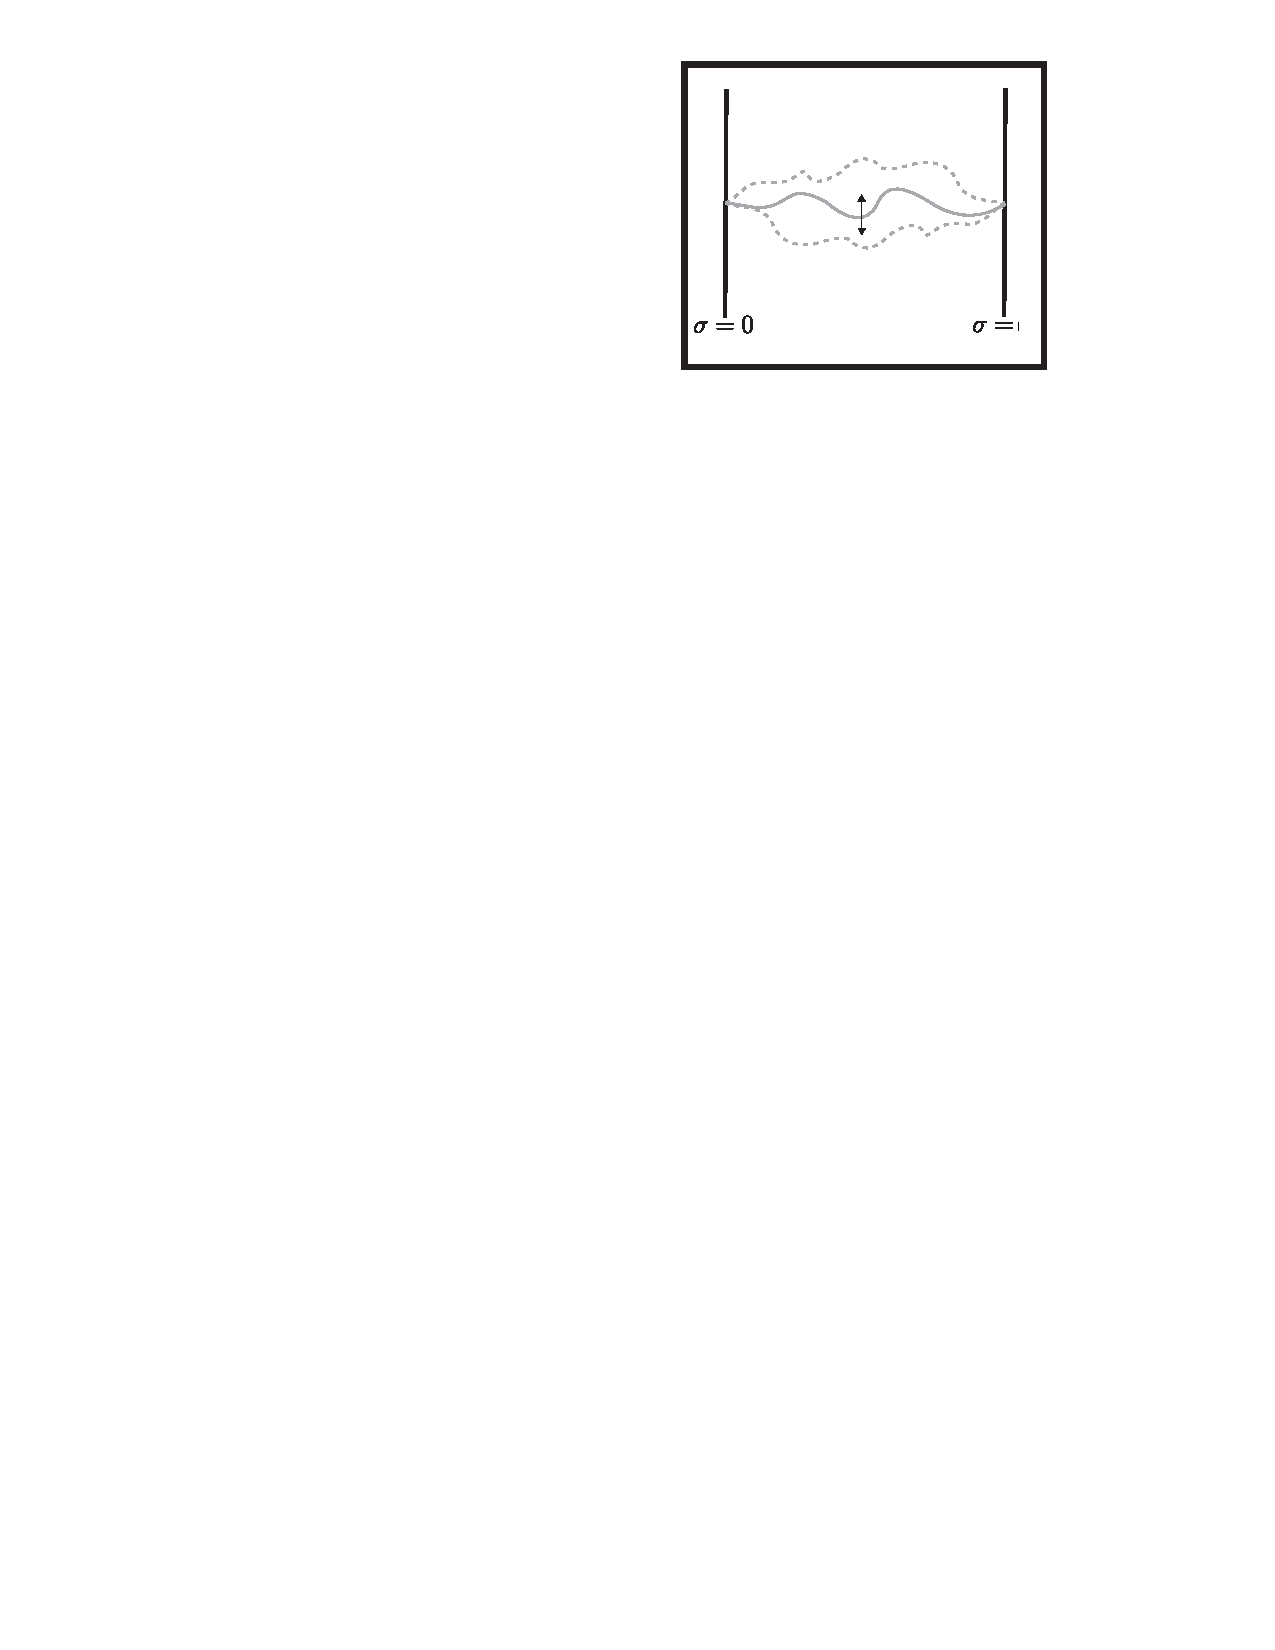
\includegraphics[width=\linewidth]{figure/string-BD}
		\caption{Dirichlet BC’s: The string can oscillate, but its endpoints are fixed at the boundary. The $y$ axis is spacetime direction $X^i$ whereas $x$ axis is worldsheet direction $\sigma$.}
		\label{fig:dirichlet}
	\end{minipage}
	\hfill
	\begin{minipage}[t]{0.48\linewidth}
		\centering
		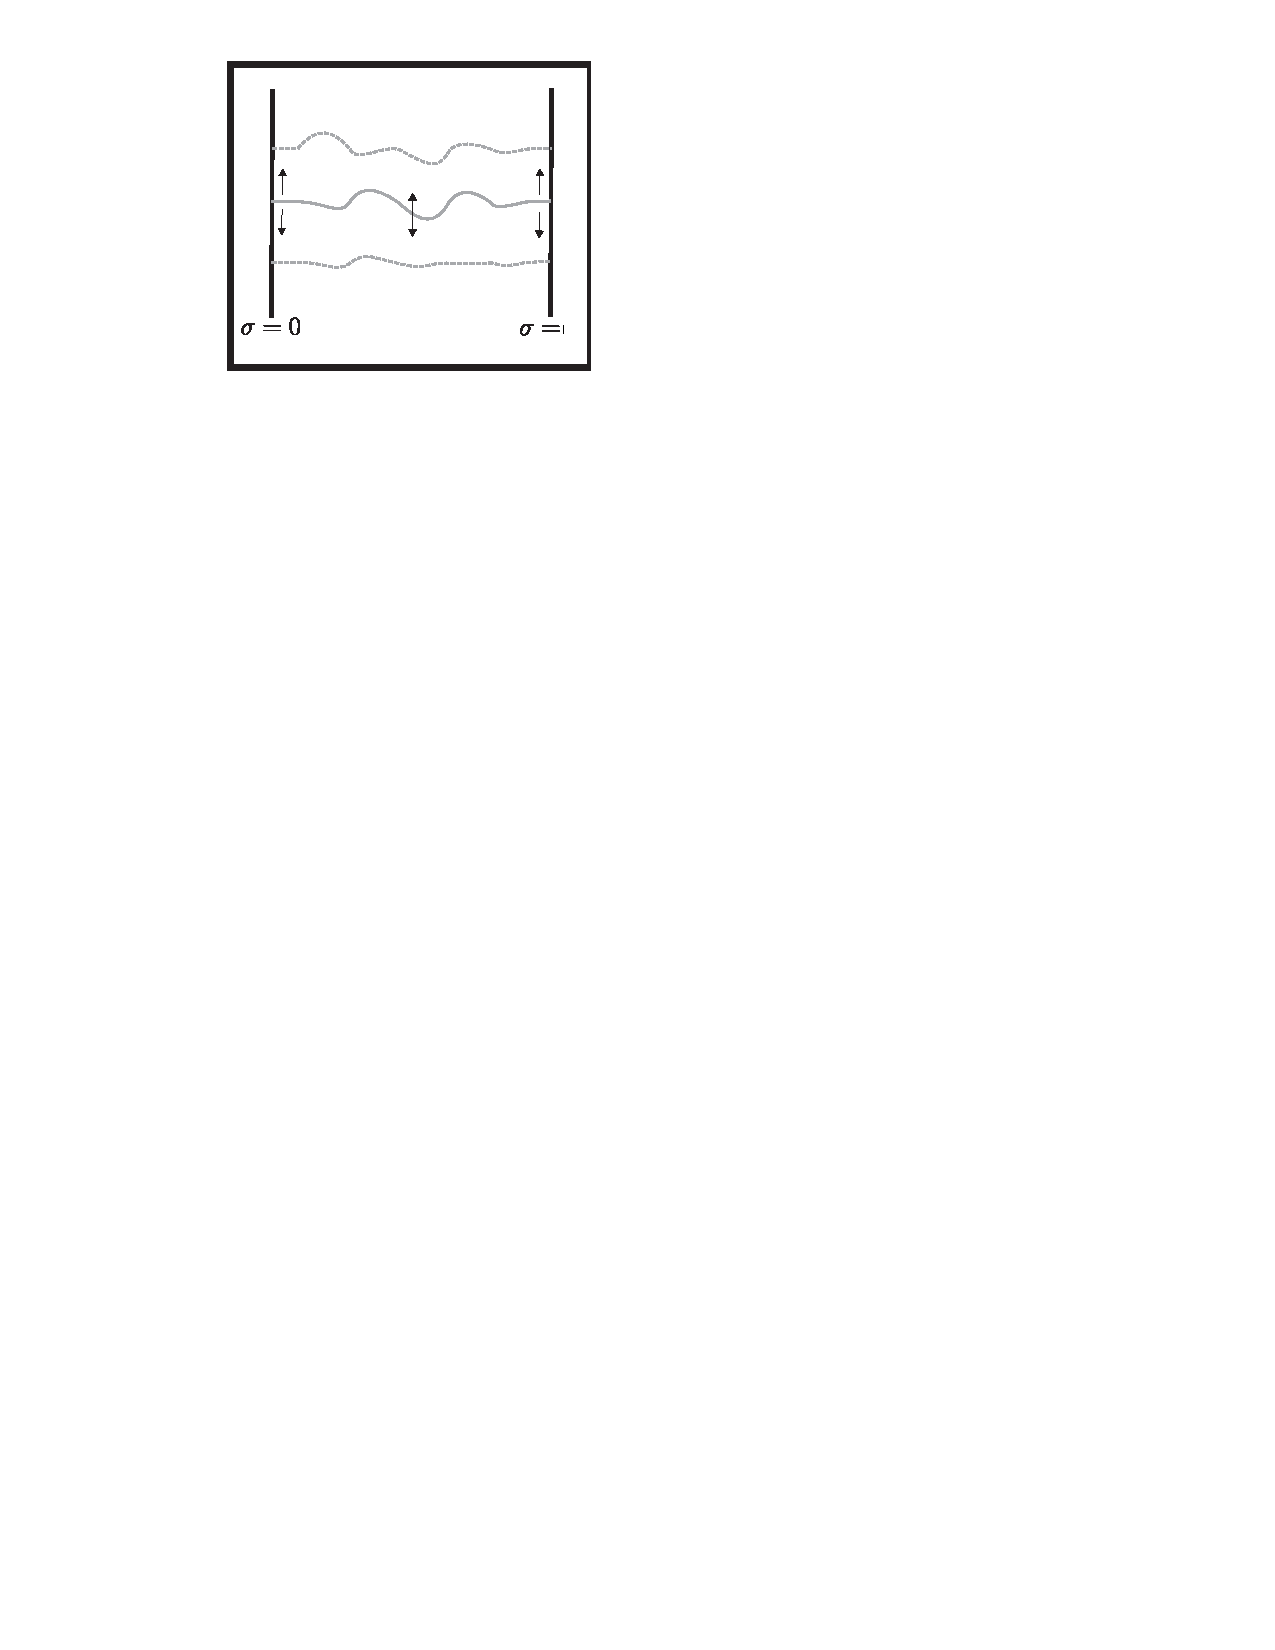
\includegraphics[width=\linewidth]{figure/string-BD1}
		\caption{Neumann BC’s: The string can oscillate and its endpoints can move along the boundaries, as long as their derivatives vanish at the boundaries. }
		\label{fig:neumann}
	\end{minipage}
\end{figure*}
The first two conditions are the only possibilities consistent with $D$-dimensional Poincaré invariance and the equations of motion. The NG and Polyakov actions are perhaps the simplest actions with the given symmetries. But simplicity is not the correct criterion; symmetry is key. 

Now we generalize the Polyakov action, requiring that the symmetries are preserved and that the action is a polynomial in derivatives. 
Global Weyl invariance, i.e., $\omega(\tau, \sigma)=C$ (where $C$ is a constant), requires that $\gamma^{ab}$ appears one more time than $\gamma_{ab}$ to cancel the variation of $(-\gamma)^{1/2}$. Additional upper indices can only contract with derivatives, so each term must have two derivatives. 
Coordinate invariance and Poincaré invariance allow: 
\begin{equation}
	\chi=\frac{1}{4 \pi} \int_{M} \dif \tau \dif \:\sigma(-\gamma)^{1 / 2} R \label{Poincar\'{e}-x}
\end{equation}
where $R$ is the Ricci scalar. 
Under a local Weyl scaling: 
\begin{equation}
	\left(-\gamma^{\prime}\right)^{1 / 2} R^{\prime}=(-\gamma)^{1 / 2}\left(R-2 \nabla^{2} \omega\right)\label{Ricci-Weyl}
\end{equation}
\begin{tcolorbox}[breakable]
	\begin{proof}
		\begin{align*}
			R^\prime &= e^{-2\omega} R - 2 e^{-3\omega} g^{\rho\sigma} \nabla_{\rho} \partial_{\sigma} e^{\omega} + 2 e^{-4\omega} g^{\rho\sigma} (\partial_{\rho} e^{\omega})(\partial_{\sigma} e^{\omega}) \\
			\intertext{Using the chain rule for the scalar $e^{\omega}$, we have $\partial_{\sigma} e^{\omega} = e^{\omega} \partial_{\sigma} \omega$ and $\nabla_{\rho} \partial_{\sigma} e^{\omega} = e^{\omega} (\partial_{\rho} \omega \partial_{\sigma} \omega + \nabla_{\rho} \partial_{\sigma} \omega)$. Substituting these:}
			R^\prime &= e^{-2\omega} R - 2 e^{-3\omega} \left[ e^{\omega} \left( g^{\rho\sigma} \partial_{\rho} \omega \partial_{\sigma} \omega + \square \omega \right) \right] + 2 e^{-4\omega} \left( e^{2\omega} g^{\rho\sigma} \partial_{\rho} \omega \partial_{\sigma} \omega \right) \\
			&= e^{-2\omega} R - 2 e^{-2\omega} (\partial \omega)^2 - 2 e^{-2\omega} \square \omega + 2 e^{-2\omega} (\partial \omega)^2 \\
			&= e^{-2\omega} (R - 2 \square \omega)
		\end{align*}
	\end{proof}
\end{tcolorbox} 
\noindent In (\ref{Ricci-Weyl}), the variation is a total derivative because for any $v^a$, we have $(-\gamma)^{1/2}\nabla_a v^a=\partial_a[(-\gamma)^{1/2}v^a]$. Thus (\ref{Poincar\'{e}-x}) is invariant for a worldsheet without boundaries. With boundaries, there is an extra surface term. 

We can include $\chi$ in the action: 
\begin{equation}
	\begin{aligned}
		S_{\mathrm{P}}^{\prime} &=S_{\mathrm{P}}-\lambda \chi \\
		&=-\int_{M} \dif \tau \dif \sigma\:(-\gamma)^{1 / 2}\left(\frac{1}{4 \pi \alpha^{\prime}} \gamma^{a b} \partial_{a} X^{\mu} \partial_{b} X_{\mu}+\frac{\lambda}{4 \pi} R\right)
	\end{aligned}
\end{equation}
This is the most general (diff $\times$ Weyl)-invariant and Poincaré-invariant action. 
$S_{\mathrm{P}}^\prime$ looks like the Hilbert action $\int (-\gamma)^{1/2}R$ for the (gravitational) metric minimally coupled to $D$ massless scalar fields. However, in 2D, the Hilbert action depends only on the topology of the worldsheet; its variation is $R_{ab}-\frac{1}{2}\gamma_{ab}R$. In 2D, the symmetries of the curvature tensor imply $R_{ab}=\frac{1}{2}\gamma_{ab}R$. The Hilbert action is invariant under continuous transformations of the metric, but has global effects. 
\begin{tcolorbox}
	\begin{remark}
		In 2D, we have $R_{abcd}= \frac{R}{2}\left(\gamma_{ac}\gamma_{bd} - \gamma_{ad}\gamma_{bc}\right)$ and as a result:
		\begin{align}
			R_{ab} &= \gamma^{cd} R_{acbd}= \frac{R}{2}\,\gamma^{cd}\left(\gamma_{ac}\gamma_{bd} - \gamma_{ad}\gamma_{bc}\right)= \frac{R}{2}\left(\delta^d_a \gamma_{bd} - \delta^c_a \gamma_{bc}\right) \nonumber\\[6pt]
			&= \frac{R}{2}\,\gamma_{ab}.
		\end{align} 
	\end{remark}
\end{tcolorbox}

\section{\texorpdfstring{The open string spectrum}{The open string spectrum}}  \label{sec:1.3}
Introduce light-cone coordinates in spacetime: 
\begin{equation}
	x^{\pm}=2^{-1 / 2}\left(x^{0} \pm x^{1}\right), \quad x^{i},\quad  i=2, \ldots, D-1
\end{equation}
Spacetime coordinates are written as $X^\mu$, and fields on the worldsheet are written as $X^\mu(\tau, \sigma)$. 
In these coordinates, the metric is: 
\begin{subequations} \label{1.3.2} %
	\begin{align}
		&a^{\mu} b_{\mu}=-a^{+} b^{-}-a^{-} b^{+}+a^{i} b^{i} \\
		&a_{-}=-a^{+}, \quad a_{+}=-a^{-}, \quad a_{i}=a^{i}
	\end{align} 
\end{subequations}
Let the worldsheet parameter $\tau$ be the spacetime coordinate $X^+$. Then $X^+$ plays the role of time, and $p^-$ is the energy. The longitudinal components $X^-, p^+$ act like spatial coordinates and momentum, as do the transverse $X^i, p^i$. 
Starting from the point particle, using $S_{\mathrm{pp}}^\prime$: 
Fix the worldline parameterization via: 
\begin{equation}
	X^+(\tau)=\tau
\end{equation}
The action becomes: 
\begin{equation}
	S_{\mathrm{pp}}^{\prime}=\frac{1}{2} \int \dif\tau\left(-2 \eta^{-1} \dot{X}^{-}+\eta^{-1} \dot{X}^{i} \dot{X}^{i}-\eta m^{2}\right)
\end{equation}
\begin{tcolorbox}
	\begin{remark}
		Here we used $\dot{X}^{\mu} \dot{X}_{\mu}=-\dot{X}^{+} \dot{X}^{-}-\dot{X}^{+} \dot{X}^{-}+\dot{X}^{i} \dot{X}^{i}=-2 \dot{X}^{-}+\dot{X}^{i} \dot{X}^{i}$. 
	\end{remark}
\end{tcolorbox}
\noindent The canonical momentum $p_{\mu}=\partial L / \partial \dot{X}^{\mu}$ is: 
\begin{equation}
	p_{-}=-\eta^{-1}, \quad p_{i}=\eta^{-1} \dot{X}^{i}
\end{equation}
Using the metric $p^i=p_i$ and $p^+=-p_-$, the Hamiltonian is: 
\begin{equation}
	\begin{aligned}
		H &=p_{-} \dot{X}^{-}+p_{i} \dot{X}^{i}-L \\
		&=-\eta^{-1}\dot{X}^s +\eta p_i p^i +\eta^{-1}\dot{X}^s -\tfrac{1}{2}\eta p_i p_i +\tfrac{1}{2}\eta m^2 \\
		&=\frac{p^{i} p^{i}+m^{2}}{2 \eta^{-1}}=\frac{p^{i} p^{i}+m^{2}}{2 p^{+}}\label{string-H}
	\end{aligned}
\end{equation}
There is no $p_+ X^+$ term because $X^+$ is not a dynamical variable. 
Furthermore, $\dot{\eta}$ does not appear in the action, so $p_\eta=0$. Since $\eta=-1/p_{-}$, we should not treat $\eta$ as an independent canonical coordinate. 

For quantization, impose canonical commutators on the dynamical fields: 
\begin{equation}
	\left[p_{i}, X^{j}\right]=-\mi \delta_{i}^{j}, \quad\left[p_{-}, X^{-}\right]=-\mi
\end{equation}
The momentum eigenstates $|k_-, k^i\rangle$ form a complete set. The remaining momentum components are determined by other quantities. The gauge choice associates $\tau$ with $X^+$, so $H=-p_+ =p^-$. The negative sign between $H$ and $p_+$ is because the former is active and the latter is passive. Thus, (\ref{string-H}) becomes the relativistic mass-shell condition. We have obtained the spectrum of a relativistic scalar. 

Turning to the open string. The coordinate region is $-\infty<\tau<+\infty$ and $0\leq \sigma\leq l$. Choose the following gauge fixing condition to remove Polyakov redundancies. Let: 
\begin{subequations} 
	\begin{align} 
		X^+&=\tau \label{1.3.8a} \\
		\partial_{\sigma} \gamma_{\sigma \sigma}&=0 \label{1.3.8b} \\
		\operatorname{det} \gamma_{a b}&=-1 \label{1.3.8c}
	\end{align}   \label{1.3.8}
\end{subequations}
How to obtain this gauge? 
First, choose $\tau$ according to (\ref{1.3.8a}). Note that $f=\gamma_{\sigma \sigma}\left(-\operatorname{det} \gamma_{a b}\right)^{-1 / 2}$ transforms as: 
\begin{equation}
	f^{\prime} \dif \sigma^{\prime}=f \dif \sigma\label{1.3.9}
\end{equation}
\begin{tcolorbox}[breakable]
	\begin{proof}
		Under a coordinate transformation $x^a \to x'^a$, the metric transforms as
		\begin{equation}
			\gamma_{ab}
			= \frac{\partial x'^c}{\partial x^a}
			\frac{\partial x'^d}{\partial x^b}
			\gamma'_{cd} \, .
		\end{equation}
		with $x^a=(\sigma,\tau)$. In matrix form this may be written as
		\begin{equation}
			\gamma = J^{\mathrm T} \, \gamma' \, J \, ,
		\end{equation}
		where $J^c{}_a = \partial x'^c / \partial x^a$ is the Jacobian matrix. Taking determinants, and using $\det(J^{\mathrm T}) = \det(J)$, we obtain
		\begin{equation}
			\det \gamma 
			= \det(J^{\mathrm T}) \, \det(\gamma') \, \det(J)
			= (\det J)^2 \det \gamma' \, .
		\end{equation}
		
		For the specific transformation $\tau' = \tau$, $\sigma' = \sigma'(\sigma,\tau)$, the Jacobian takes the triangular form
		\begin{equation}
			J =
			\begin{pmatrix}
				\displaystyle \frac{\partial \sigma'}{\partial \sigma} & \displaystyle \frac{\partial \sigma'}{\partial \tau} \\
				0 & 1
			\end{pmatrix} \, ,
		\end{equation}
		so that
		\begin{equation}
			\det J = \frac{\partial \sigma'}{\partial \sigma} \, .
		\end{equation}
		Hence,
		\begin{equation}
			\det \gamma
			= \left(\frac{\partial \sigma'}{\partial \sigma}\right)^2 \det \gamma' \, .
		\end{equation}
		One can prove \eqref{1.3.9} together with the following
		\begin{align}
			\gamma_{\sigma'\sigma'}&=\pdv{\sigma}{\sigma'}\pdv{\sigma}{\sigma'}\gamma_{\sigma\sigma}\\
			\dif \sigma'&=\pdv{\sigma'}{\sigma}\dif \sigma
		\end{align}
	\end{proof}
\end{tcolorbox}
Define the invariant length $\dif l=f\dif \sigma$. Define the $\sigma$ coordinate of a point proportional to the invariant length from $\sigma=0$ to that point. The proportionality constant is determined by keeping the right endpoint at $\sigma=l$. In this coordinate system, $f=\dif l/\dif \sigma$ is independent of $\sigma$, though it may depend on $\tau$. 
Finally, perform a Weyl transformation to satisfy (\ref{1.3.8c}). Since $f$ is Weyl-invariant, $\partial_\sigma f$ remains zero. Combined with (\ref{1.3.8c}), this implies $\partial_{\sigma} \gamma_{\sigma \sigma}=0$, so (\ref{1.3.8b}) is also satisfied. 

For $\gamma_{\tau\tau}(\tau, \sigma)$, we can solve the gauge condition (\ref{1.3.8c}). Since $\gamma_{\sigma\sigma}$ is independent of $\sigma$, the only independent degrees of freedom in the metric are now $\gamma_{\sigma\sigma}(\tau)$ and $\gamma_{\sigma\tau}(\tau, \sigma)$. 
The inverse metric is: 
\begin{equation}
	\begin{bmatrix}
		\gamma^{\tau \tau} & \gamma^{\tau \sigma} \\
		\gamma^{\sigma \tau} & \gamma^{\sigma \sigma}
	\end{bmatrix}=
	\begin{bmatrix}
		-\gamma_{\sigma \sigma}(\tau) & \gamma_{\tau \sigma}(\tau, \sigma) \\
		\gamma_{\tau \sigma}(\tau, \sigma) & \gamma_{\sigma \sigma}^{-1}(\tau)\left(1-\gamma_{\tau \sigma}^{2}(\tau, \sigma)\right)
	\end{bmatrix}
\end{equation}
\begin{tcolorbox}[breakable]
	\begin{proof}
		\[
		\begin{bmatrix}
			\gamma_{\tau \tau} & \gamma_{\tau \sigma} \\
			\gamma_{\tau \sigma} & \gamma_{\sigma\sigma}
		\end{bmatrix}
		\begin{bmatrix}
			\gamma^{\tau\tau} & \gamma^{\tau \sigma} \\
			\gamma^{\tau \sigma} & \gamma^{\sigma \sigma}
		\end{bmatrix}
		=\begin{bmatrix}
			-\gamma_{\tau \tau} \gamma_{\sigma \sigma}+\gamma_{\tau \sigma}^{2} &  \gamma_{\tau\tau} \gamma_{\tau \sigma}+\gamma_{\tau \sigma} \gamma_{\sigma \sigma}^{-1}\left(1-\gamma_{\tau \sigma}^{2}\right) \\
			-\gamma_{\sigma \sigma} \gamma_{\tau \sigma}+\gamma_{\sigma \sigma} \gamma_{\tau \sigma} & \gamma_{\tau \sigma}^{2}+1-\gamma_{\tau \sigma}^{2}  
		\end{bmatrix}
		\]
		Then use (\ref{1.3.8c}) given by $\gamma_{\tau\tau} \gamma_{\sigma \sigma}-\gamma_{\tau \sigma}^{2}=-1$. 
	\end{proof} 
\end{tcolorbox}
\noindent Thus, the Polyakov Lagrangian becomes: 
\begin{equation}
	\begin{aligned}
		L&=-\frac{1}{4 \pi \alpha^{\prime}} \int_{0}^{\ell} \dif\sigma\: \Bigl[\gamma_{\sigma \sigma}\left(2 \partial_{\tau} x^{-}-\partial_{\tau} X^{i} \partial_{\tau} X^{i}\right) \\
		&\qquad \quad-2 \gamma_{\sigma \tau}(\partial_{\sigma} Y^{-}-\partial_{\tau} X^{i} \partial_{\sigma} X^{i})
		+\gamma_{\sigma \sigma}^{-1}(1-\gamma_{\tau \sigma}^{2}) \partial_{\sigma} X^{i} \partial_{\sigma} X^{i}\Bigr]
	\end{aligned}
\end{equation}
\begin{tcolorbox}[breakable]
	\begin{proof}
		Expand the Polyakov action (\ref{1.2.13}) by components:
		\begin{align*}
			L=-\frac{1}{4 \pi \alpha^{\prime}} \int_{0}^{\ell} \dif\sigma \:\Bigl[-\gamma_{\sigma \sigma}\underbrace{(\partial_\tau X^{\mu} \partial_\tau X_{\mu})}_{(1)} 
			+2 \gamma_{\tau \sigma}\underbrace{(\partial_{\tau} X^{\mu} \partial_{\sigma} X_{\mu})}_{(2)} 
			+\gamma_{\sigma \sigma}^{-1}(1-\gamma_{\tau \sigma}^{2}) \underbrace{(\partial_{\sigma} X^{\mu} \partial_{\sigma} X_{\mu})}_{(3)}\Bigr] 
		\end{align*}
		where
		\begin{align*}
			(1) &=-\dot{X}^{+} \dot{X}^{-}-\dot{X}^{+} \dot{X}^{-}+\dot{X}^{i} \dot{X}^{i} =-2 \partial_{\tau} X^{-}+\partial_{\tau} X^{i} \partial_{\tau} X^{i} \\
			(2) &=-\partial_{\tau} X^{\dagger} \partial_{\sigma} X^{-}-\partial_{\tau} X^{-} \partial_{\sigma} X^{+}+\partial_{\tau} X^{i} \partial_{\sigma} X^{i} \\
			&=-\partial_{\sigma} X^{-}-\partial_{\tau} X^{-} \partial_{\sigma} \tau+\partial_{\tau} X^{i} \partial_{\tau} X^{i} =-\left(\partial_{\sigma} Y^{-}-\partial_{\tau} X^{i} \partial_{\sigma} X^{i}\right) \\
			(3) &=-\partial_{\sigma} X^{-} \partial_{\sigma} X^{+}-\partial_{\sigma} X^{+} \partial_{\sigma} X^{-}+\partial_{\sigma} X^{i} \partial_{\sigma}X^{i} 
			=\partial_{\sigma} X^{i} \partial_{\sigma} X^{i}
		\end{align*}
		Q.E.D. 
	\end{proof}
\end{tcolorbox}
\noindent Here we split $X^-(\tau, \sigma)$ into two parts: $x^-(\tau)$ and $Y^-(\tau, \sigma)$. $x^-(\tau)$ is the average value of $X^-$ at time $\tau$. 
\begin{subequations}
	\begin{align}
		x^{-}(\tau)&=\frac{1}{\ell} \int_{0}^{\ell} \dif \sigma X^{-}(\tau, \sigma) \\
		Y^{-}(\tau, \sigma)&=X^{-}(\tau, \sigma)-x^{-}(\tau)
	\end{align}
\end{subequations}
$Y^-$ does not appear in terms containing time derivatives and is thus non-dynamical. It acts like a Lagrange multiplier, constraining $\partial_\sigma \gamma_{\tau\sigma}$ to be zero. 
Under gauge (\ref{1.3.8}), the open string boundary condition (\ref{Neumann-bound}) becomes: 
\begin{equation}
	\gamma_{\tau \sigma} \partial_{\tau} X^{\mu}-\gamma_{\tau \tau} \partial_{\sigma} X^{\mu}=0 \quad \text { at } \sigma=0, \ell
\end{equation}
\begin{proof}
	$
	\partial^{\sigma} X^{\mu} =\gamma^{\sigma a} \partial_{a} X^{\mu}=\gamma^{\sigma \tau} \partial_{\tau} X^{\mu}+\gamma^{\sigma \sigma} \partial_{\sigma} X^{\mu} =\gamma_{\tau \sigma} \partial_{\tau} X^{\mu}+\gamma_{\sigma \sigma}^{-1}\left(1-\gamma_{\tau \sigma}^{2}\right) \partial_{\sigma} X^{\mu} =\gamma_{\tau \sigma} \partial_{\tau} X^{\mu}-\gamma_{\tau \tau} \partial_{\sigma} X^{\mu}
	$
	Q.E.D. 
\end{proof}
\noindent For $\mu=+$: 
\begin{equation}
	\gamma_{\tau \sigma}=0 \quad \text { at } \sigma=0, \ell
\end{equation}
Since $\partial_\sigma \gamma_{\tau\sigma}=0$, $\gamma_{\tau\sigma}$ vanishes everywhere. 
For $\mu=i$, the boundary condition is: 
\begin{equation}
	\partial_{\sigma} X^{i}=0 \quad \text { at } \sigma=0, \ell   \label{bound-mu-i}
\end{equation}
Imposing gauge conditions and including the Lagrange multiplier $Y^-$, the Lagrangian is: 
\begin{equation}
	L=-\frac{\ell}{2 \pi \alpha^{\prime}} \gamma_{\sigma \sigma} \partial_{\tau} x^{-}+\frac{1}{4 \pi \alpha^{\prime}} \int_{0}^{\ell} \dif\sigma\,\Bigl(\gamma_{\sigma \sigma} \partial_{\tau} X^{i} \partial_{\tau} X^{i}-\gamma_{\sigma \sigma}^{-1} \partial_{\sigma} X^{i} \partial_{\sigma} X^{i}\Bigr)
\end{equation}
The conjugate momentum to $x^-$ is: 
\begin{equation}
	p_{-}=-p^{+}=\frac{\partial L}{\partial\left(\partial_{\tau} x^{-}\right)}=-\frac{\ell}{2 \pi \alpha^{\prime}} \gamma_{\sigma \sigma}\label{1.3.17}
\end{equation}
As with the einbein $\eta$ in the particle case, $\gamma_{\sigma\sigma}$ is momentum rather than a coordinate. 
The conjugate momentum density to $X^i(\tau, \sigma)$ is: 
\begin{equation}
	\Pi^{i}=\frac{\delta L}{\delta\left(\partial_{\tau} X^{i}\right)}=\frac{1}{2 \pi \alpha'} \gamma_{\sigma \sigma} \partial_{\tau} X^{i}=\frac{p^{+}}{\ell} \partial_{\tau} X^{i} \label{1.3.18}
\end{equation}
Thus, the Hamiltonian is: 
\begin{align}
	H &=p_{-} \partial_{\tau} x^{-}-L+\int_{0}^{\ell} \dif \sigma\: \Pi_{i} \partial_{\tau} X^{i} \nonumber \\
	&= p_{-} \partial_{\tau}  x^{-}-p_{-} \partial_{\tau} x^{-} -\frac{1}{4 \pi \alpha^{\prime}} \int_{0}^{\ell} \dif \sigma\:\biggl(\gamma_{\sigma \sigma} \partial_{\tau} X^{i} \partial_{\tau} X^{i}-\frac{\partial_{\sigma} X^{i} \partial_{\sigma} X^{i}}{\gamma_{\sigma \sigma}}\biggr) 
	+\int_{0}^{\ell} \dif \sigma\: \frac{\ell\,\Pi_{i}^{2} }{ p^{+}} \nonumber \\
	&=\frac{\ell}{4 \pi \alpha^{\prime} p^{+}} \int_{0}^{\ell} \dif \sigma\, 4 \pi \alpha^{\prime}\Pi_{i}^{2} -\frac{\gamma_{\sigma\sigma}^{-1}}{4 \pi \alpha^{\prime}} \int_{0}^{\ell} \dif \sigma\,\Bigl(\left(2 \pi \alpha^{\prime} \Pi^{i}\right)^{2}-\partial_\sigma X^{i} \partial _\sigma X^{i} \Bigr)\nonumber \\
	&=\frac{\ell}{4 \pi \alpha^{\prime} p^{+}} \int_{0}^{\ell} d \sigma\left(2 \pi \alpha^{\prime} \Pi^{i} \Pi^{i}+\frac{1}{2 \pi \alpha^{\prime}} \partial_{\sigma} X^{i} \partial_{\sigma} X^{i}\right) \label{1.3.19}
\end{align}
This is precisely the Hamiltonian for $D-2$ free fields $X^i$, where $p^+$ is a conserved quantity. 
The equations of motion are: 
\begin{subequations}
	\begin{align}
		\partial_{\tau} x^{-}&=\frac{\partial H}{\partial p_-}=-\frac{\partial H}{\partial p^{+}}=-\frac{H p^{+} \partial(p^+)^{-1}}{\partial p^{+}}=\frac{H}{p^+} \:,\quad
		\partial_{\tau} p^{+}=\frac{\partial H}{\partial x^{-}}=0 \\
		\partial_{\tau} X^{i}&=\frac{\delta H}{\delta \Pi^{i}}=\frac{\ell}{2 p^{+}} 2 \Pi^{i}=2 \pi\alpha^{\prime}c\Pi^{i} \:,\quad
		\partial_\tau \Pi^{i}=-\frac{\delta H}{\delta X^{i}}=\frac{c}{2 \pi \alpha^{\prime}} \partial_{\sigma}^{2} X^{i} \:,
	\end{align}
\end{subequations}
where $c=\ell/(2 \pi \alpha^{\prime} p^{+})$. 
This leads to the wave equation: 
\begin{equation}
	\partial_{\tau}^{2} X^{i}=c^{2} \partial_{\sigma}^{2} X^{i}
\end{equation}
Choose $\ell$ such that $c=1$. Thus $p^+$ is conserved, and the total string length $\ell$ remains constant. 

$X^\pm$ also satisfy the wave equation. $X^-$ requires some calculation. Under (\ref{bound-mu-i}), the general solution to the wave equation is: 
\begin{equation}
	X^{i}(\tau, \sigma)=x^{i}+\frac{p^{i}}{p^{+}} \tau+\mi\left(2 \alpha^{\prime}\right)^{1 / 2} \sum_{n=-\infty \atop n \neq 0}^{\infty} \frac{1}{n} \alpha_{n}^{i} \exp \left(-\frac{\pi \mi n c \tau}{\ell}\right) \cos \frac{\pi n \sigma}{\ell} \label{1.3.22}
\end{equation}
where we write the expansion coefficient $A_n=\sqrt{2\alpha'}\frac{\alpha_n^i}{n}$ to make \eqref{1.3.25b} cleaner and the purpose of $\sqrt{2\alpha'}$ factor is to make the constants $\alpha_n^i$ dimensionless. The reality of $X^i$ requires $\alpha_{-n}^{i}=\left(\alpha_{n}^{i}\right)^{\dagger}$. 
Define center-of-mass variables: 
\begin{subequations}
	\begin{align}
		x^{i}(\tau)&=\frac{1}{\ell} \int_{0}^{\ell} \dif \sigma\: X^{i}(\tau, \sigma) \\
		p^{i}(\tau)&=\int_{0}^{\ell} \dif \sigma\: \Pi^{i}(\tau, \sigma)=\frac{p^{+}}{\ell} \int_{0}^{\ell} \dif \sigma \:\partial_{\tau} X^{i}(\tau, \sigma)
	\end{align}
\end{subequations}
These represent the average mass and total momentum. These are Heisenberg operators. 
In (\ref{1.3.22}), they are Schrödinger operators $x^{i} \equiv x^{i}(0)$ and $p^{i} \equiv p^{i}(0)$. 
For quantization, impose commutation relations: 
\begin{subequations}
	\begin{align}
		\left[x^{-}, p^{+}\right]&=\mi \eta^{-+}=-\mi  \label{1.3.24a}\\
		\left[X^{i}(\sigma), \Pi^{j}\left(\sigma^{\prime}\right)\right]&=\mi \delta^{i j} \delta\left(\sigma-\sigma^{\prime}\right)
		\label{1.3.24b}
	\end{align}
\end{subequations}
Written in terms of Fourier components: 
\begin{subequations}
	\begin{align}
		\left[x^{i}, p^{j}\right]&=\mi \delta^{i j}   \label{1.3.25a}\\
		\left[\alpha_{m}^{i}, \alpha_{n}^{j}\right]&=m \delta^{i j} \delta_{m,-n}   \label{1.3.25b}
	\end{align} \label{1.3.25}
\end{subequations}
\noindent For each $m$ and $i$, the modes satisfy the harmonic oscillator algebra: 
\begin{equation}
	\alpha_{m}^{i} \sim m^{1 / 2} a, \quad \alpha_{-m}^{i} \sim m^{1 / 2} a^{\dagger}, \quad m>0
\end{equation}
where $[a, a^\dagger]=1$. 
\begin{tcolorbox}[breakable]
	\begin{proof}
		Equations (\ref{1.3.24b}), (\ref{1.3.25a}), and (\ref{1.3.25b}) form a logical loop; knowing any two allows derivation of the third. 
		Assume the latter two are known to prove the first. Introduce the notation:
		\[\sideset{}{'}\sum={\sum_{n=-\infty\atop n \neq 0}^{+\infty} }\]
		From (\ref{1.3.18}) and (\ref{1.3.22}), we have:
		\begin{align}
			\Pi^{i}(\tau, \sigma)
			=&\frac{p^{i}}{\ell}+\frac{p^+}{\ell}\mi \left(2 \alpha^{\prime}\right)^{1 / 2} \sideset{}{'}\sum \frac{1}{n} \alpha_{n}^{i}\left(-\frac{\pi \mi n c}{\ell}\right) \exp \left(-\frac{\pi \mi n c \tau}{\ell}\right) \cos \frac{n \pi \sigma}{\ell} \nonumber \\
			=&\frac{p^ i}{\ell}+\frac{1}{\left(2 \alpha^{\prime}\right)^{1 / 2} \ell} \sideset{}{'}\sum \alpha_{n}^{i} \exp \left(-\frac{\pi \mi n c\tau}{\ell}\right) \cos \frac{n \pi \sigma}{\ell} \tag{1.a} \label{1.a}
		\end{align}
		where we used:
		\[
		\mi\left(2 \alpha^{\prime }\right)^{1 / 2} \frac{-\mi \pi c}{\ell}=\pi\left(2 \alpha^{\prime}\right)^{1 / 2} \frac{1}{2 \alpha^{\prime} \pi p^{+}}=\frac{1}{(2 \alpha^\prime)^{1 / 2} p^{+}}
		\]
		Then:
		\[
		[X^{i} , \Pi^{i}]=\frac{1}{\ell}\left[x^{i} , p^{i}\right]+\frac{\mi}{\ell } \sideset{}{'}\sum_{n,m} \frac{1}{n} \exp \left(-\frac{\pi \mi n c \tau}{\ell}\right) \cos \frac{n \pi \sigma}{\ell}
		\left[\alpha_{n}^{i}, \alpha_{m}^{i}\right] \exp \left(-\frac{\pi \mi m c \tau}{\ell}\right) \cos \frac{m \pi \sigma^\prime}{\ell}
		\]
		Let $\left[\alpha_{m}^{i}, \alpha_{n}^{i}\right]=m \delta_{m,-n}$. Given the completeness relation:
		\[
		2\pi\delta(\sigma^{\prime}-\sigma)=\sum_{n=-\infty}^{+\infty} \me^{ \mi n\left(\sigma^{\prime}-\sigma\right)}
		=1+\sideset{}{'}\sum \me^{  \mi n \left(\sigma^{\prime}-\sigma\right)}
		\]
		The latter term becomes:
		\begin{align*}
			&\quad -\frac{\mi}{\ell} {\sum}^\prime \frac{1}{n} \exp \left(-\frac{\pi \mi n c \tau}{\ell}\right) \cos \frac{n \pi \sigma}{\ell}(-n)  \exp \left(+\frac{\pi \mi n c \tau}{\ell}\right) \cos \frac{-n \pi \sigma^\prime}{\ell}\\
			&=\frac{\mi}{\ell} {\sum}^\prime \cos\frac{n \pi \sigma}{\ell} \cos \frac{n \pi \sigma^{\prime}}{\ell} \\
			&=\frac{\mi}{ 4\ell}  {\sum}^\prime \Bigl[\me^{\mi n \pi(\sigma+\sigma^{\prime})/\ell}+\me^{-\mi n \pi(\sigma+\sigma^{\prime})/\ell}+ \me^{\mi n \pi(\sigma-\sigma^{\prime})/\ell}+\me^{-\mi n \pi(\sigma-\sigma^{\prime})/\ell}\Bigr]\\
			&=\frac{\mi}{2\ell} \Bigl( 2\pi\delta\bigl(\pi(\sigma+\sigma^{\prime})/\ell\bigr)-1+2\pi\delta\bigl(\pi(\sigma-\sigma^{\prime})/\ell\bigr)-1 \Bigr) \\
			&=-\frac{\mi}{\ell}+\frac{\mi \pi}{ \ell} \delta\bigl(\pi(\sigma-\sigma^{\prime})/\ell\bigr) 
			=-\frac{\mi}{\ell}+\mi \delta(\sigma-\sigma^{\prime})
		\end{align*}
		Note $\delta(\sigma-\sigma^\prime)=\delta(\sigma^\prime-\sigma)$, giving a factor of 2; and $\sigma, \sigma^\prime>0$ makes $\delta\bigl(\pi(\sigma+\sigma^{\prime})/\ell\bigr)=0$. 
		Since $[x^{i}, p^{i}]=\mi$, we have:
		$$\left[X^{i} , \Pi^{i}\right]=\mi \delta(\sigma-\sigma^{\prime})$$ 
		Q.E.D.
	\end{proof}
\end{tcolorbox}
The state $|0;k \rangle$ (where $k=(k^+, k^i)$) is annihilated by lowering operators and is an eigenstate of the center-of-mass momentum: 
\begin{subequations}
	\begin{align}
		p^{+}|0 ; k\rangle&=k^{+}|0 ; k\rangle, \quad p^{i}|0 ; k\rangle=k^{i}|0 ; k\rangle \\
		\alpha_{m}^{i}|0 ; k\rangle&=0, \quad m>0
	\end{align}
\end{subequations}
General states are obtained by acting with raising operators on $|0;k \rangle$: 
\begin{equation}
	|N ;  k\rangle=\left[\prod_{i=2}^{D-1} \prod_{n=1}^{\infty} \frac{\left(\alpha_{-n}^{i}\right)^{N_{i n}}}{\left(n^{N_{i n}} N_{i n} !\right)^{1 / 2}}\right]|0 ; k\rangle\label{general-state}
\end{equation}
Independent states can be labeled by center-of-mass momenta $k^+, k^i$ and occupation numbers $N_{in}$. Center-of-mass momentum represents the point particle degrees of freedom, while oscillators represent infinite internal degrees of freedom. From a spacetime view, each choice of occupation numbers corresponds to a different particle state or spin. States (\ref{general-state}) form the single open string Hilbert space $\mathscr{H}$. 
In particular, state $|0;0 \rangle$ is the ground state of a single string with zero momentum, not the vacuum state without strings. We call the latter $|\text{vacuum} \rangle$. Operators acting on it cannot create or annihilate strings, but only act on the state space of individual strings. The $n$-string Hilbert space $\mathscr{H}_n$ is formed by the product of $n$ spaces of (\ref{general-state}); wave functions must be symmetric, as all these states have integer spin (to be proven). 
In the free limit, the total Hilbert space of string theory is: 
\begin{equation}
	\mathscr{H}=\lvert \text{vacuum}\rangle \oplus \mathscr{H}_{1} \oplus \mathscr{H}_{2} \oplus \ldots
\end{equation}
Substituting (\ref{1.3.22}) into (\ref{1.3.19}) yields: 
\begin{equation}
	H=\frac{p^{i} p^{i}}{2 p^{+}}+\frac{1}{2 p^{+} \alpha^{\prime}}\left(\sum_{n=1}^{\infty} \alpha_{-n}^{i} \alpha_{n}^{i}+A\right)
\end{equation}
\begin{tcolorbox}[breakable]
	\begin{proof}
		First, split the string Hamiltonian (\ref{1.3.19}) into two parts:
		\begin{align*}
			H_{\Pi}=\frac{\ell}{2 p^+} \int_{0}^{\ell} \dif \sigma \: \Pi^{i} \Pi^{i}\:, \quad 
			H_{X}=\frac{\ell}{2p^{+}(2 \pi \alpha^\prime)^{2} } \int_{0}^{\ell} \dif \sigma \:\partial_{\sigma} X^{i} \partial_{\sigma} X^{i} \:. 
		\end{align*}  
		Using (\ref{1.a}), we have:
		\begin{align*}
			H_\Pi&=\frac{\ell}{2 p^+} \int_{0}^{\ell} \dif \sigma \:
			\Biggl( \frac{p^{i} p^{i}}{\ell^{2}}
			+\frac{1}{2 \alpha^\prime \ell^2} \sideset{}{'}\sum_{n,m} \alpha_{n}^{i} \alpha_{m}^{i}\exp\Bigl(-\frac{\pi \mi c \tau}{\ell}(n+m)\Bigr)  \cos \frac{n \pi \sigma}{\ell} \cos \frac{m\pi \sigma}{\ell}  \\
			&\qquad \qquad\qquad  +\frac{2p^{i}}{\left(2 \alpha^{\prime}\right)^{1 / 2 } \ell^{2}} \sideset{}{'}\sum \alpha_{n}^{i} \exp \left(-\frac{\pi \mi n c \tau}{\ell}\right) \cos \frac{n \pi \sigma}{\ell} \Biggr) \\
			&=\frac{p^{i}p^{i}}{2p^{+}}+\frac{1}{4p^{+}\alpha'}\sideset{}{'}\sum_{n,m} \alpha_{n}^{i} \alpha_{m}^{i}\exp\Bigl(-\frac{\pi \mi c \tau}{\ell}(n+m)\Bigr)\bigl(\delta_{n,m}+\delta_{n,-m}\bigr)/2
		\end{align*}
		Using (\ref{1.3.22}), we have:
		\begin{align*}
			\partial_\sigma X^{i} =-\frac{\mi\left(2 \alpha^{\prime}\right)^{1 / 2} \pi}{\ell} \sideset{}{'}\sum \alpha_{n}^{i} \exp \Bigl(-\frac{\pi \mi n c \tau}{\ell}\Bigr) \sin \frac{n \pi \sigma}{\ell} \:,
		\end{align*}
		Then:
		\begin{align*}
			H_X &=\frac{\ell}{2p^{+}(2 \pi \alpha^\prime)^{2} } \frac{-2 \alpha^\prime \pi^2}{\ell^2} \int_{0}^{\ell} \dif \sigma \sideset{}{'}\sum _{n,m} \alpha_{n}^{i}\alpha_{m}^{i} 
			\exp \Bigl(-\frac{\pi \mi c \tau}{\ell}(n+m)\Bigr) \sin \frac{n \pi \sigma}{l}\sin \frac{m \pi \sigma}{\ell} \\
			&=-\frac{1}{4p^{+}\alpha^\prime  }  \sideset{}{'}\sum _{n,m} \alpha_{n}^{i}\alpha_{m}^{i} 
			\exp \Bigl(-\frac{\pi \mi c \tau}{\ell}(n+m)\Bigr) \bigl(\delta_{n,m}-\delta_{n,-m}\bigr)/2
		\end{align*}
		So:
		\begin{align*}
			H&=H_{\Pi}+H_{X}=\frac{p^{i}p^{i}}{2p^{+}} +\frac{1}{4p^{+}\alpha'}\sideset{}{'}\sum_{n,m} \alpha_{n}^{i} \alpha_{m}^{i}\exp\Bigl(-\frac{\pi \mi c \tau}{\ell}(n+m)\Bigr)\delta_{n,-m} \\
			&=\frac{p^{i}p^{i}}{2p^{+}} +\frac{1}{4p^{+}\alpha'}\sideset{}{'}\sum_{m} \alpha_{-m}^{i} \alpha_{m}^{i}
		\end{align*}
		And:
		\begin{align*}
			\sum_{n} \alpha_{-n}^{i} \alpha_{n}^{i}&=\sum_{n=-\infty}^{-1} \alpha_{-n}^{i} \alpha_{n}^{i}+\sum_{n=1}^{\infty} \alpha_{-n}^{i} \alpha_{n}^{i}=\sum_{n=\infty}^{1} \alpha_{n}^{i} \alpha_{-n}^{i}+\sum_{n=1}^{\infty} \alpha_{-n}^{i} \alpha_{n}^{i}=\sum_{n=1}^{\infty} (\alpha_{n}^{i} \alpha_{-n}^{i}+\alpha_{-n}^{i} \alpha_{n}^{i})\\
			&=2 \sum_{n=1}^{\infty} \alpha_{-n}^{i} \alpha_{n}^{i}+\sum_{n=1}^{\infty} n\delta^{ii}=2 \sum_{n=1}^{\infty} \alpha_{-n}^{i} \alpha_{n}^{i}+(D-2)\sum_{n=1}^{\infty} n
		\end{align*}
		Since $i=2,3...,D-1$, thus $A=(D-2)\sum_{n=1}^{\infty}n/2=(D-2)\zeta(-1)/2$. 
		Q.E.D.
	\end{proof}
\end{tcolorbox}
\noindent In this $H$, the operator ordering is ambiguous. We have placed lowering operators on the right and raising operators on the left. The constant $A$ in Hamiltonian arises from the commutators. In the detailed treatment of light-cone quantization, the constant is determined as follows: the choice of light-cone gauge obstructs the theory's Lorentz invariance. By seeking the generator of Lorentz transformations $M^{\mu\nu}$ and verifying its algebra with $p^\mu$ and other operators, only one case is consistent: $A=-1$. The corresponding spacetime dimension is $D=26$. 

In light-cone quantization, we do not wish to dwell too much on this. We will obtain the values of $A$ and $D$ using conformal gauge methods. It will show us why incorrect values of $A$ and $D$ in the light-cone method lose Lorentz invariance. 
First, we consider the operator ordering constant in the Hamiltonian to originate from the sum of zero-point energies of each oscillator mode. 
For a bosonic field like $X^\mu$, this is $\omega/2$. The expressions $\frac{1}{2} \omega\left(a a^{\dagger}+a^{\dagger} a\right)$ and $\omega\left(a^{\dagger} a+\frac{1}{2}\right)$ are equivalent. In $H$: 
\begin{equation}
	A=\frac{D-2}{2} \sum_{n=1}^{\infty} n \:, \label{1.3.31}
\end{equation}
where $D-2$ comes from the sum over transverse directions. This zero-point energy diverges. Using renormalization techniques: 
\begin{equation}
	\sum_{n=1}^{\infty} n \rightarrow-\frac{1}{12} \:.  \label{1.3.32}
\end{equation}
To obtain this, insert a smooth cutoff factor: 
\begin{equation}
	\exp (-\epsilon \gamma_{\sigma \sigma}^{-1 / 2}|k_{\sigma}|)=	\exp \left(-\frac{n\pi\epsilon}{\sqrt{\gamma_{\sigma\sigma}}\ell}\right) \label{1.3.33}
\end{equation}
where $k_\sigma=n\pi/\ell$. The factor $\gamma_{\sigma\sigma}^{-1/2}$ ensures invariance under $\sigma$ reparameterization $(dl=\int_{0}^{\ell} \sqrt{\gamma_{\sigma\sigma}}d\sigma=\sqrt{\gamma_{\sigma\sigma}}\int_0^{\ell}d\sigma)$. 
\begin{equation}
	\begin{aligned}
		A & \rightarrow \frac{D-2}{2} \sum_{n=1}^{\infty} n \exp \left[-\epsilon n\left(\pi / 2 p^{+} \alpha^{\prime} \ell\right)^{1 / 2}\right]\\
		&=\frac{D-2}{2}\left(\frac{2 \ell p^{+} \alpha^{\prime}}{\epsilon^{2} \pi}-\frac{1}{12}+O(\epsilon)\right)
	\end{aligned}
\end{equation}
The first term of the cutoff is proportional to the string length $\ell$ and can be canceled by counterterms in the action proportional to $\int \dif^2\sigma(-\gamma)^{1/2}$. 
In fact, Weyl invariance $\gamma_{\sigma\sigma}\to e^{2\omega}\gamma_{\sigma\sigma}$ requires it to be canceled, leaving only the cutoff-independent second term: 
\begin{equation}
	A=\frac{2-D}{24}
\end{equation}
\begin{tcolorbox}
	\begin{proof}
		From \eqref{1.3.17} we have $\gamma_{\sigma\sigma}=\frac{2\pi\alpha'p^{+}}{\ell}$ thus \eqref{1.3.31} becomes:
		\begin{equation}
			\begin{aligned}
				A & \rightarrow \frac{D-2}{2} \sum_{n=1}^{\infty} n \exp \left[-\epsilon n\left(\pi / 2 p^{+} \alpha^{\prime} \ell\right)^{1 / 2}\right]\\
				&=-\frac{D-2}{2} \dv{[\epsilon\left(\pi / 2 p^{+} \alpha^{\prime} \ell\right)^{1 / 2}]}\sum_{n=1}^{\infty} \exp \left[-\epsilon n\left(\pi / 2 p^{+} \alpha^{\prime} \ell\right)^{1 / 2}\right]
			\end{aligned}
		\end{equation}
		This is geometric series and the summation is known to be:
		\begin{equation}
			\begin{aligned}
				&=\frac{D-2}{2} \dv{\epsilon\left(\pi / 2 p^{+} \alpha^{\prime} \ell\right)^{1 / 2}}\left[\frac{1}{1-\exp \left[\epsilon\left(\pi / 2 p^{+} \alpha^{\prime} \ell\right)^{1 / 2}\right]}\right]\\
				&=\frac{D-2}{2}\left(\frac{2 \ell p^{+} \alpha^{\prime}}{\epsilon^{2} \pi}-\frac{1}{12}+O(\epsilon)\right)=\frac{D-2}{2}\left(\frac{\gamma_{\sigma\sigma}\ell^2}{\pi^2\epsilon^2}-\frac{1}{12}+O(\epsilon)\right)\\
				&=\frac{D-2}{2}\left(\frac{(\sqrt{\gamma_{\sigma\sigma}}dl)^2}{\pi^2\epsilon^2}-\frac{1}{12}+O(\epsilon)\right)
			\end{aligned}
		\end{equation}
	\end{proof}
\end{tcolorbox}
The finite residue is an example of Casimir energy, which arises because the string length is finite. For a point particle $p^-=H$, so: 
\begin{equation}
	m^{2}=2 p^{+} H-p^{i} p^{i}=\frac{1}{\alpha^{\prime}}\left(N+\frac{2-D}{24}\right)
\end{equation}
where $N$ is the level: 
\begin{equation}
	N=\sum_{i=2}^{D-1} \sum_{n=1}^{\infty} n N_{i n}
\end{equation}
The mass of each state is determined by its excitation level. Consider some light string states. The lightest is: 
\begin{equation}
	|0 ; k\rangle, \quad m^{2}=\frac{2-D}{24 \alpha^{\prime}}
\end{equation}
If $D>2$, $m^2$ is negative, and this state is a tachyon. 
In field theory, the scalar potential is $\frac{1}{2}m^2\phi^2$, so a negative mass squared implies that the "no-string" vacuum is actually unstable, similar to symmetric states in spontaneous symmetry breaking. Whether the bosonic string has any stable vacuum is a complex question, and the answer remains unclear. For superstrings, there are "tachyon-free" theories. We will continue to use the bosonic string as a model for developing string techniques, ignoring this instability. 

The lowest excited state of the string is the excitation of the $n=1$ mode once: 
\begin{equation}
	\alpha_{-1}^{i}|0 ; k\rangle, \quad m^{2}=\frac{26-D}{24 \alpha^{\prime}}
\end{equation}
Lorentz invariance imposes requirements on $D$. For massless and massive particles, the spin analysis is different. For massive particles, in the rest frame $p^\mu=(m, 0, \cdots, 0)$. 
Then the internal states form a representation of the spatial rotation group $SO(D-1)$. For massless particles, there is no rest frame; we choose a frame $p^\mu=(E, E, 0, \cdots, 0)$. Then $SO(D-2)$ acts on the transverse dimensions leaving $p^\mu$ invariant, and internal states form a group representation. For $D=4$, a massive particle is labeled by spin $j$, an $SO(3)$ representation, so there are $2j-1$ states. A massless particle is labeled by helicity $\lambda$, an eigenstate under a single generator of $SO(2)$. Lorentz invariance requires only this one state, but $\mathsf{CPT}$ symmetry imposes $\lambda$ and $-\lambda$. 
In $D$ dimensions, a massive particle has $D-1$ spin states, while a massless particle has $D-2$ states. In the first level, we only find $D-2$ states $\alpha_{-1}^{i}|0 ;  k\rangle$, so it must be massless. 
\begin{equation}
	A=-1,\quad D=26
\end{equation}
This is a striking and important result. Only when the spacetime dimension $D=26$ is the spectrum Lorentz-invariant. The classical theory is Lorentz-invariant for any $D$, but there is an anomaly: except for $D=26$, quantization does not preserve Lorentz invariance. 

Light-cone quantization picks out two directions, leaving $SO(D-2)$ acting on the transverse dimensions. For the transverse directions, the spin generator is: 
\begin{equation}
	S^{i j}=-\mi \sum_{n=1}^{\infty} \frac{1}{n}(\alpha_{-n}^{i} \alpha_{n}^{j}-\alpha_{-n}^{j} \alpha_{n}^{i})
\end{equation}
It is antisymmetric in $i, j$, and together with Lorentz invariance, forbids zero-point energy constants for massless states. 
\begin{tcolorbox}[breakable]
	\begin{proof}
		$S^{ij}$ is defined as $S^{ij}= \int_{0}^{\ell}\dif\sigma\: X^{i}\Pi^{j}-X^{j}\Pi^{i}$. Note that at this point $p_{i}=0$, so:
		\begin{equation*}
			X^{i} \Pi^{j}-X^{j}\Pi^{i}=\frac{\mi}{\ell} \sideset{}{'}\sum_{n, m} \frac{1}{n} \alpha_{n}^{i} \alpha_{m}^{j} \exp \Bigl(-\frac{\pi \mi c \tau}{\ell}(n+m)\Bigr) \cos \frac{n \pi \sigma}{\ell} \cos \frac{m \pi \sigma}{\ell} -(i\leftrightarrow j). 
		\end{equation*}
		From this, it follows:
		\begin{align*}
			S^{ij}&=\mi\sideset{}{'}\sum_{n, m} \frac{1}{n} \alpha_{n}^{i} \alpha_{m}^{j} \exp \Bigl(-\frac{\pi \mi c \tau}{\ell}(n+m)\Bigr)\bigl(\delta_{n,m}+\delta_{n,-m}\bigr)/2-(i\leftrightarrow j) \\
			&=\frac{\mi}{2}\sideset{}{'}\sum_{n} \frac{1}{n} \alpha_{n}^{i} \alpha_{-n}^{j}-\frac{1}{n} \alpha_{n}^{j} \alpha_{-n}^{i}\\
			&=\frac{\mi}{2}\left(\sum_{n=-\infty}^{-1} \frac{1}{n} \alpha_{n}^{i} \alpha_{-n}^{j}-\frac{1}{n} \alpha_{n}^{j} \alpha_{-n}^{i}\right)+\frac{\mi}{2}\left(\sum_{n=1}^{\infty} \frac{1}{n} \alpha_{n}^{i} \alpha_{-n}^{j}-\frac{1}{n} \alpha_{n}^{j} \alpha_{-n}^{i}\right)\\
			&=\frac{\mi}{2}\sum_{n=1}^{\infty} -\frac{1}{n}\mathcolor{red}{\alpha_{-n}^{i} \alpha_{n}^{j}}+\frac{1}{n}\mathcolor{blue}{ \alpha_{-n}^{j} \alpha_{n}^{i}}+ \frac{1}{n} \mathcolor{blue}{\alpha_{n}^{i} \alpha_{-n}^{j}}-\frac{1}{n} \mathcolor{red}{\alpha_{n}^{j} \alpha_{-n}^{i}}
		\end{align*}
		Since $S^{ii}=0$ and $[\alpha^i_m,\alpha^j_n]=0$ for $i\ne j$, we have:
		\begin{align*}
			S^{ij}&=-\mi\sum_{n=1}^{\infty} \frac{1}{n} (\alpha_{-n}^{i} \alpha_{n}^{j}- \alpha_{-n}^{j} \alpha_{n}^{i})
		\end{align*}
		Q.E.D. 
	\end{proof}
\end{tcolorbox}

For a massless particle, by choosing the momentum direction to be the "1" direction selected by quantization, the entire $SO(D-2)$ spin symmetry is made manifest. 
For massive particles, only an $SO(D-2)$ subgroup is obvious within the $SO(D-1)$ symmetry of light-cone quantization. But this is still useful. 
Under the action of $SO(D-2)$ on the transverse directions, the vector representation of $SO(D-1)$ breaks into an invariant and a $(D-2)$-vector: 
\begin{equation}
	\mathbf{v}=\left(v^{1}, 0, \ldots, 0\right)+\left(0, v^{2}, \ldots, v^{D-1}\right)
\end{equation}
Thus, if a massive particle is in the vector representation of $SO(D-1)$, when we examine its transformation properties under $SO(D-2)$, we will see a scalar and a vector. Higher excited states of the string are massive, forming full representations of $SO(D-1)$. 
At level $N$, the maximum eigenvalue of the spin component $S^{23}$ is $N$, obtained by acting $N$ times with $\alpha_{-1}^{2}+\mi \alpha_{-1}^{3}$. 
Therefore: 
\begin{equation}
	S^{23} \leq 1+\alpha^{\prime} m^{2}
\end{equation}
\begin{tcolorbox}[breakable]
	We start by checking the Eigenvalue of $S^{23}$ for the state $(\alpha^2_{-m} + i\alpha^3_{-m}) |0;k\rangle$ for a given $m$:
	\begin{align}
		S^{23} (\alpha^2_{-m} + i\alpha^3_{-m}) |0;k\rangle 
		&= -i \sum_{n=1}^{\infty} \frac{1}{n} (\alpha^2_{-n} \alpha^3_n - \alpha^3_{-n} \alpha^2_n)(\alpha^2_{-m} + i\alpha^3_{-m}) |0;k\rangle \nonumber \\[6pt]
		&= -\frac{i}{m} (\alpha^2_{-m} \alpha^3_m - \alpha^3_{-m} \alpha^2_m)(\alpha^2_{-m} + i\alpha^3_{-m}) |0;k\rangle \nonumber \\[6pt]
		&= -\frac{i}{m} (\alpha^2_{-m} \alpha^3_m i\alpha^3_{-m} - \alpha^3_{-m} \alpha^2_m \alpha^2_{-m}) |0;k\rangle \nonumber \\[6pt]
		&= (\alpha^2_{-m} + i\alpha^3_{-m}) |0;k\rangle
		\tag{1.53}
	\end{align}
	
	where we have used $[\alpha^i_m,\alpha^j_n] = m\delta^{ij}\delta_{m+n,0}$ and $\alpha_{m}^i|0\rangle=0$. 	So this state has spin one. Consider now
	\begin{align}
		S^{23} (\alpha^2_{-m} + i\alpha^3_{-m})^2 |0;k\rangle 
		&= -i \sum_{n=1}^{\infty} \frac{1}{n} (\alpha^2_{-n}\alpha^3_n - \alpha^3_{-n}\alpha^2_n)(\alpha^2_{-m} + i\alpha^3_{-m})^2 |0;k\rangle \nonumber \\[6pt]
		&= -\frac{i}{m} (\alpha^2_{-m}\alpha^3_m - \alpha^3_{-m}\alpha^2_m)(\alpha^2_{-m} + i\alpha^3_{-m})^2 |0;k\rangle \nonumber \\[6pt]
		&= -\frac{i}{m} (\alpha^2_{-m}\alpha^3_m - \alpha^3_{-m}\alpha^2_m)
		(\alpha^2_{-m}\alpha^2_{-m}+ i\alpha^2_{-m}\alpha^3_{-m} + i\alpha^3_{-m}\alpha^2_{-m} \nonumber\\
		&\qquad - \alpha^3_{-m}\alpha^3_{-m}) |0;k\rangle \nonumber \\[6pt]
		&= 2(\alpha^2_{-m}\alpha^2_{-m} + i\alpha^2_{-m}\alpha^3_{-m} + i\alpha^3_{-m}\alpha^2_{-m} - \alpha^3_{-m}\alpha^3_{-m}) |0;k\rangle \nonumber \\[6pt]
		&= 2(\alpha^2_{-m} + i\alpha^3_{-m})^2 |0;k\rangle
		\tag{1.54}
	\end{align}
	
	Similarly we find
	\begin{align}
		S^{23} (\alpha^2_{-m} + i\alpha^3_{-m})^N |0;k\rangle 
		= N (\alpha^2_{-m} + i\alpha^3_{-m})^N |0;k\rangle
		\tag{1.55}
	\end{align}
	
	Any other state at level $N$ will contain at least one less factor of 
	$\alpha^2_{-m} + i\alpha^3_{-m}$ and as $S^{23}$ only has non-zero Eigenvalue 
	on that specific combination, it will give a spin lower than $N$. 
	Using the mass-shell condition (1.3.36) on $D=26$, i.e. $\alpha' m^2 = N - 1$ 
	we thus find
	\begin{align}
		S^{23} \le N = \alpha' m^2 + 1
		\tag{1.56}
	\end{align}
	QED.
\end{tcolorbox}
The slope in the inequality is called the Regge slope. Meson resonances follow this form of linear relationship, i.e., $\alpha^{\prime} \sim(1 \mathrm{GeV})^{-2}$. For this reason, string theory was originally a theory of strong interactions in the 1970s. Now, as a theory of quantum gravity, $\alpha^\prime$ is on the order of $M_P^{-2}$, and the mass of massive particles is on the order of $M_P$. 
It is so large that at current experimental levels, these particles only appear as virtual states. Therefore, we are particularly interested in the massless string spectrum. 
Most known particles have mass, but it is so small compared to $M_P$ that it is zero to first approximation, becoming non-zero due to small symmetry breaking. 

\section{\texorpdfstring{Closed and unoriented strings}{Closed and unoriented strings}} \label{sec:1.4}
Light-cone quantization of the closed string is very similar to the open string. Again, impose gauge conditions (\ref{1.3.8a})-(\ref{1.3.8c}). For the open string, these completely determine the gauge. 
For the closed string, some additional coordinate freedom remains: 
\begin{equation}
	\sigma^{\prime}=\sigma+s(\tau) \bmod \ell
\end{equation}
Since $\sigma=0$ can be chosen as any point on the string, most of this residual freedom can be fixed by an extra gauge condition: 
\begin{equation}
	\gamma_{\tau \sigma}(\tau, 0)=0
\end{equation}
i.e., the line $\sigma=0$ is perpendicular to the lines $\tau=C$ (where $C$ is a constant). Except for a global translation, this completely determines the line $\sigma=0$. Thus, (1.3.8) and (1.4.2), except for a $\tau$-independent translation of $\sigma$, fix all gauge freedom. 
\begin{equation}
	\sigma^{\prime}=\sigma+s \bmod \ell   \label{sigma-translation}
\end{equation}
The analysis now parallels the open string: Lagrangian, canonical momentum, Hamiltonian, equations of motion, etc. General periodic solutions to the equations of motion: 
\begin{equation}
	\begin{aligned}
		X^{i}(\tau, \sigma) &=x^{i}+\frac{p^{i}}{p^{+}} \tau+\mi\left(\frac{\alpha^{\prime}}{2}\right)^{1 / 2} \\
		& \times \sum_{n=-\infty \atop n \neq 0}^{\infty}\left\{\frac{\alpha_{n}^{i}}{n} \exp \left[-\frac{2 \pi \mi n(\sigma+c \tau)}{\ell}\right]+\frac{\tilde{\alpha}_{n}^{i}}{n} \exp \left[\frac{2 \pi \mi n(\sigma-c \tau)}{\ell}\right]\right\} \label{general-periodic-solution}
	\end{aligned}
\end{equation}
In the closed string, there are two sets of independent oscillatory solutions $\alpha_{n}^{i}, \tilde{\alpha}_{n}^{i}$, corresponding to waves moving left and right along the string. 
In the open string, boundary conditions at the ends mix these. The independent degrees of freedom are again transverse oscillations and center-of-mass variables for both transverse and longitudinal directions: 
\begin{equation}
	\alpha_{n}^{i}, \tilde{\alpha}_{n}^{i}, x^{i}, p^{i}, x^{-}, p^{+}
\end{equation}
with canonical commutators: 
\begin{subequations}
	\begin{align}
		\left[x^{-}, p^{+}\right]&=-\mi \\
		\left[x^{i}, p^{j}\right]&=\mi \delta^{i j} \\
		\left[\alpha_{m}^{i}, \alpha_{n}^{j}\right]&=m \delta^{i j} \delta_{m,-n} \\
		\left[\tilde{\alpha}_{m}^{i}, \tilde{\alpha}_{n}^{j}\right]&=m \delta^{i j} \delta_{m,-n} 
	\end{align}
\end{subequations}
Starting from the state $|0,0;k \rangle$, which has center-of-mass momentum $k^\mu$ and is annihilated by $\alpha_{n}^{i}, \tilde{\alpha}_{n}^{i}$ for $m>0$. 
General states are: 
\begin{equation}
	|N, \tilde{N} ; k\rangle=\left[
	\prod_{i=2}^{D-1} \prod_{n=1}^{\infty} \frac{(\alpha_{-n}^{i})^{N_{i n}}(\tilde{\alpha}_{-n}^{i})^{\tilde{N}_{i n}}}{(n^{N_{i n}} N_{i n}! n^{\tilde{N}_{i n}} \tilde{N}_{i n}!)^{1 / 2}}
	\right] |0,0 ;  k\rangle
\end{equation}
The mass formula is: 
\begin{equation}
	\begin{aligned}
		m^{2} &=2 p^{+} H-p^{i} p^{i} \\
		&=\frac{2}{\alpha^{\prime}}\left[\sum_{n=1}^{\infty}\left(\alpha_{-n}^{i} \alpha_{n}^{i}+\tilde{\alpha}_{-n}^{i} \tilde{\alpha}_{n}^{i}\right)+A+\tilde{A}\right] \\
		&=\frac{2}{\alpha^{\prime}}(N+\tilde{N}+A+\tilde{A})
	\end{aligned}
\end{equation}
We split levels and zero-point energies into two parts: left-moving and right-moving. Summing zero-point energies gives: 
\begin{equation}
	A=\tilde{A}=\frac{2-D}{24}
\end{equation}
Due to the residual gauge freedom, i.e., the $\sigma$ translation in (\ref{sigma-translation}), there is an additional constraint. 
The operator generating $\sigma$ translations is: 
\begin{equation}
	\begin{aligned}
		P &=-\int_{0}^{\ell} \dif \sigma \:\Pi^{i} \partial_{\sigma} X^{i} \\
		&=-\frac{2 \pi}{\ell}\left[\sum_{n=1}^{\infty}\left(\alpha_{-n}^{i} \alpha_{n}^{i}-\tilde{\alpha}_{-n}^{i} \tilde{\alpha}_{n}^{i}\right)+A-\tilde{A}\right] \\
		&=-\frac{2 \pi}{\ell}(N-\tilde{N})
	\end{aligned}
\end{equation}
States must satisfy: 
\begin{equation}
	N=\tilde{N}
\end{equation}
The lightest closed string state: 
\begin{equation}
	|0,0 ; k\rangle, \quad m^{2}=\frac{2-D}{6 \alpha^{\prime}}
\end{equation}
is also a tachyon. 
The first excited state: 
\begin{equation}
	\alpha_{-1}^{i} \tilde{\alpha}_{-1}^{j}|0,0 ; k\rangle, \quad m^{2}=\frac{26-D}{6 \alpha^{\prime}} \label{1-excited-state}
\end{equation}
As with the open string, these states do not add up to a full representation of $SO(D-1)$, so the level must be massless: 
\begin{equation}
	A=\tilde{A}=-1, \quad D=26
\end{equation}
State (\ref{1-excited-state}) transforms as a 2nd-rank tensor under $SO(D-2)$. This is a reducible representation. It can be decomposed into a symmetric traceless tensor, an antisymmetric tensor, and a scalar. 
That is, any tensor $e^{ij}$ can be split into: 
\begin{equation}
	e^{i j}=\frac{1}{2}\left(e^{i j}+e^{j i}-\frac{2}{D-2} \delta^{i j} e^{k k}\right)+\frac{1}{2}\left(e^{i j}-e^{j i}\right)+\frac{1}{D-2} \delta^{i j} e^{k k} \label{1.4.15}
\end{equation}
These three separate terms do not mix under rotation. 
\begin{tcolorbox}
	\begin{remark}
		\begin{align*}
			&(\ref{1.4.15})= \\
			&\frac{1}{2}\left(\alpha_{-1}^{i} \tilde{\alpha}_{-1}^{j}+\tilde{\alpha}_{-1}^{j} \tilde{\alpha}_{-1}^{i}-\frac{2}{D-2} \delta^{i j} \alpha_{-1}^{k} \tilde{\alpha}_{-1}^{k}\right)
			+\frac{1}{2}\left(\alpha_{-1}^{i} \tilde{\alpha}_{-1}^{j}-\alpha_{-1}^{j} \tilde{\alpha}_{-1}^{i}\right)
			+\frac{1}{D-2} \delta^{i j} \alpha_{-1}^{k} \tilde{\alpha}_{-1}^{k} 
		\end{align*}
	\end{remark}
\end{tcolorbox}

At any energy level, $N_{in}$ and $\tilde{N}_{in}$ are independent except for the $N=\tilde{N}$ constraint. 
Therefore, the closed string spectrum at $m^{2}=4(N-1)/\alpha^{\prime}$ is the product of two pairs of open string levels $m^{2}=(N-1) / \alpha^{\prime}$. 

Light cone quantization was gauge fixed version, even thought $\Pi^0\ne0$, but $T^{ab}=0$ which implies $\Pi^0$ and $\Pi^i$ are not independent. Since $X^0$ comes with wrong sign, we need to eliminate $\Pi^0$. 2D diff invariance removes two classes of normal modes from the spectrum. If we attempted to build a covariant theory without this invariance, we would have to generalize the transverse commutators (\ref{1.3.25}) to: 
\begin{equation}
	\left[\alpha_{m}^{\mu}, \alpha_{n}^{\nu}\right]=m \eta^{\mu \nu} \delta_{m,-n} \label{1.4.16}
\end{equation}
Lorentz invariance forces the timelike oscillators to have a wrong-sign commutator. 
\begin{remark}
	$\left[\alpha_{m}^{\mu}, \alpha_{n}^{\nu}\right]=m \eta^{\mu \nu} \delta_{m,-n}$, so $\left[\alpha_{m}^{0}, \alpha_{-m}^{0}\right]=-m$, and
	$\alpha_{-m}^{0}={\alpha_{m}^{0}}^\dagger$. Because $\langle 0|\alpha_{m}^{0} \alpha_{-m}^{0}|  0\rangle=-m\langle 0\vert 0\rangle<0$, $\alpha_{m}^{0}\vert 0\rangle$ is a negative-norm state.
\end{remark}
\noindent States with an odd number of timelike excitations will have a negative norm. This is inconsistent with quantum mechanics. 
In fact, the theory of (\ref{1.4.16}) predates the string theory we describe, which was discovered by requiring that negative-norm states cannot be produced in physical processes. The commutator (\ref{1.4.16}) arises from covariant quantization of string theory, where coordinate invariance appears as a constraint to eliminate negative-norm states. 

The appearance of massless vectors in open string theory, and massless symmetric and antisymmetric tensors in closed string theory, is significant. General principles require a massless vector to couple to a conserved current, thus the theory has gauge invariance. 
In all fundamental string theories, this is our first example of a massless gauge particle. Actually, this particular gauge boson, called the photon, is not very interesting because the gauge group is only $U(1)$, and all particles in the theory are neutral. In Chapter 6, we will discuss a simple generalization of open string theory, adding Chan–Paton degrees of freedom at the string endpoints. This leads to $U(n)$, $SO(n)$, and $Sp(n)$ gauge groups. Similarly, massless symmetric tensor particles must couple to a conserved symmetric tensor source. The only such source is the energy-momentum tensor (with other possibilities in special cases; coupling consistent with it requires the theory to have spacetime coordinate invariance). Therefore, the massless symmetric tensor is the graviton, and general relativity is included as a small part of closed string theory. The massless antisymmetric tensor is called a 2-form gauge boson. In section 3.7, we will see that there is a local spacetime symmetry associated with it. 
In 4D, massless string states excited by 2nd and 3rd direction oscillators are identified by their helicity $\lambda=S^{23}$. The photon has $\lambda=1$, the graviton $\lambda=2$. Closed string scalars and antisymmetric tensors give $\lambda=0$ states, called the dilaton and axion, respectively. 

We conclude this section with unoriented string theory. Everything discussed previously was oriented string theory. we have not considered the coordinate transformation: 
\begin{equation}
	\sigma^{\prime}=\ell-\sigma, \quad \tau^{\prime}=\tau \label{unoriented-transformation}
\end{equation}
This changes the orientation (chirality) of the worldsheet. This symmetry is generated by the worldsheet parity operator $\Omega$. Performing (\ref{unoriented-transformation}) twice gives the identity, so $\Omega^2=1$, and eigenvalues of $\Omega$ are $\pm 1$. 
From the mode expansions (\ref{1.3.22}) and (\ref{general-periodic-solution}), we see that in the open string: 
\begin{equation}
	\Omega \alpha_{n}^{i} \Omega^{-1}=(-1)^{n} \alpha_{n}^{i}
\end{equation}
In the closed string: 
\begin{subequations}
	\begin{align}
		\Omega \alpha_{n}^{i} \Omega^{-1}&=\tilde{\alpha}_{n}^{i}\\
		\Omega \tilde{\alpha}_{n}^{i} \Omega^{-1}&=\alpha_{n}^{i}
	\end{align}
\end{subequations}
By fixing $\Omega=+1$ for the ground states $|0;k\rangle, |0,0;k\rangle$, we define the phase of $\Omega$. Later, we will see this choice is made so that $\Omega$ is conserved under interactions. Thus: 
\begin{subequations}
	\begin{align}
		\Omega|N ; k\rangle&=(-1)^{N}|N ;  k\rangle \\
		\Omega|N, \tilde{N} ; k\rangle&=|\tilde{N}, N ; k\rangle.
	\end{align}
\end{subequations}
There is a consistent interacting string theory, the unoriented string theory, in which only states with $\Omega=+1$ are retained. Focusing on massless states, the open string photon has $\Omega=-1$ and is thus forbidden in the unoriented theory. Acting on massless tensor states in the closed string, the parity operator $\Omega$ changes $e^{ij}$ into $e^{ji}$. Thus gravitons and dilatons appear in unoriented theory, but the antisymmetric tensor does not. 
Note that both open and closed string tachyons survive in unoriented theory, so we have to work harder to remove them. 

Two other constraints arise when studying interactions: 
First, it is possible to have consistent theories with only closed strings, or both closed and open strings, but not with only open strings. Closed strings can always be produced in open string scattering. 
Second, oriented or unoriented open strings can only couple with the same type of closed strings. We list possible combinations and their massless spectra. Let $G_{\mu\nu}, B_{\mu\nu}, \Phi, A_\mu$ denote the graviton, antisymmetric tensor, dilaton, and photon. 
Then: 
\begin{enumerate}
	\item Oriented bosonic closed string: $G_{\mu\nu}, B_{\mu\nu}, \Phi$.
	\item Unoriented bosonic closed string: $G_{\mu\nu}, \Phi$.
	\item Oriented bosonic closed and open strings: $G_{\mu\nu}, B_{\mu\nu}, \Phi, A_\mu$.
	\item Unoriented bosonic closed and open strings: $G_{\mu\nu}, \Phi$.
\end{enumerate}
All of these have gravitons, dilatons, and tachyons. Massless oriented open strings will be $U(n)$ gauge bosons, while massless unoriented open strings will be $SO(n)$ or $Sp(n)$ gauge bosons. 